\documentclass[11pt]{report}
\usepackage{amsmath}
\usepackage{graphicx} %to add pictures - tagged with successive numbers
\usepackage{float} %to force locate the pic in position
\usepackage{subcaption}
%\usepackage{movie15}
\usepackage{multimedia}
%\usepackage{hyperref}


% Title Page
\title{\textbf{\huge Line Follower Robot}}
\author{Ahmad Samir\\ Abderahman Shazly}


\begin{document}
	%Useful settings for pagenumbering:
	%gobble - no numbers
	%arabic - arabic numbers
	%roman - roman numbers
	
	\maketitle
	\begin{titlepage}
		\begin{center}
			\line(1,0){300}\\
			[3mm]
			\huge \bfseries Line Follower Robot\\
			[2mm]
			\line(1,0){200}\\
			[1.5cm]
			\textsc{\LARGE A DETAILED MINI-PROJECT REPORT}\\
			[0.75cm]
			\textsc{\Large AT FAB-LAB INTERNSHIP} \\	
		\end{center}
	\end{titlepage}
	
	
	\pagenumbering{gobble}
	\newpage
	\begin{titlepage}
		\line(1,0){0}\\
		[7cm]
		\huge This page was lifted Blanck \\
	\end{titlepage}
	
	\begin{abstract}
	
		
		
		Line follower is an autonomous robot which follows either black line in white area or white line in black area. Robot must be able to detect particular line and keep following it.
		\begin{figure}[ht]
			\begin{center}
				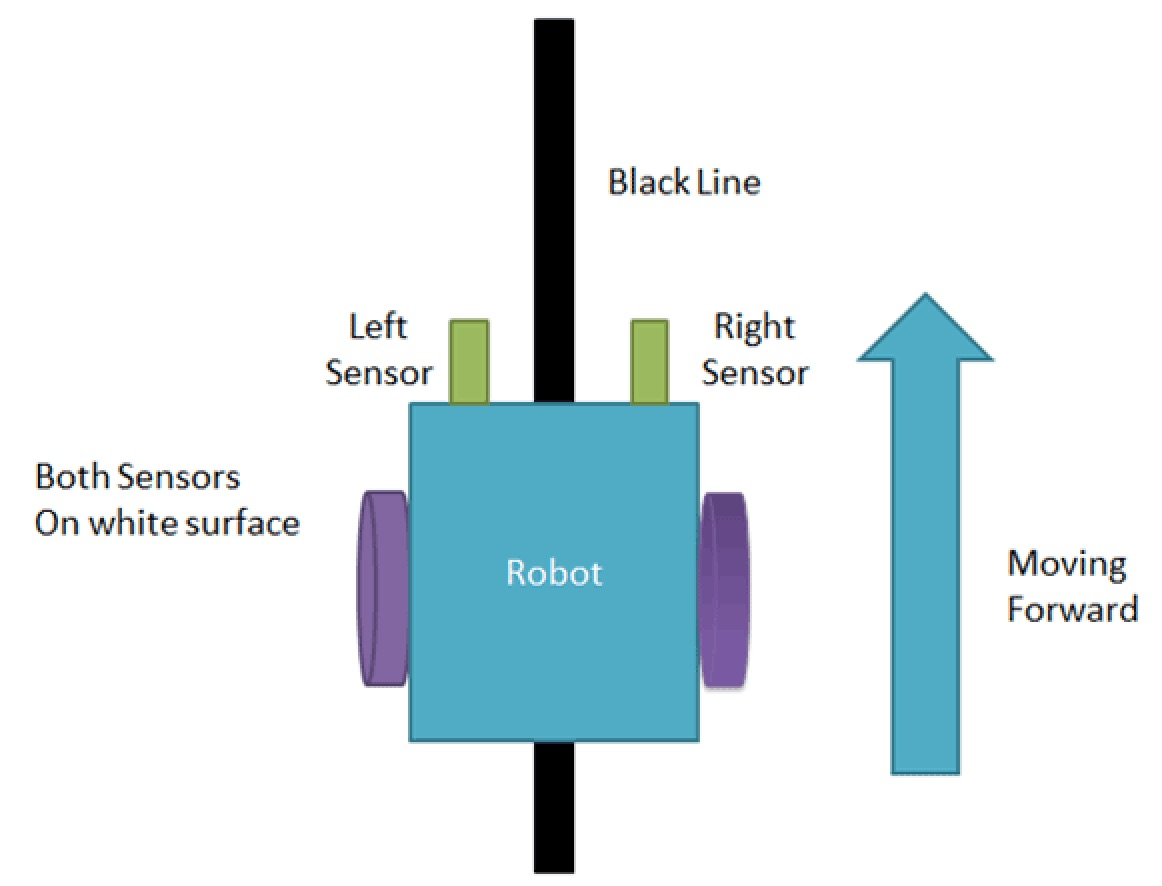
\includegraphics[scale=0.07]{Working-of-Arduino-Line-Fol.jpg}
				\caption{Working of Line Follower}
				\label{fig:fig1}
			\end{center}
		\end{figure}
		
		For special situations such as cross overs where robot can have more than one path which can be followed, predefined path must be followed by the robot.
		
		In our project , we asked to design the line follower robot to follow black line in white area and take right or left turn whenever cross overs turn arrives.
		
		\begin{figure}[ht]
			\begin{center}
					\begin{subfigure}[normal]{0.3\textwidth}
						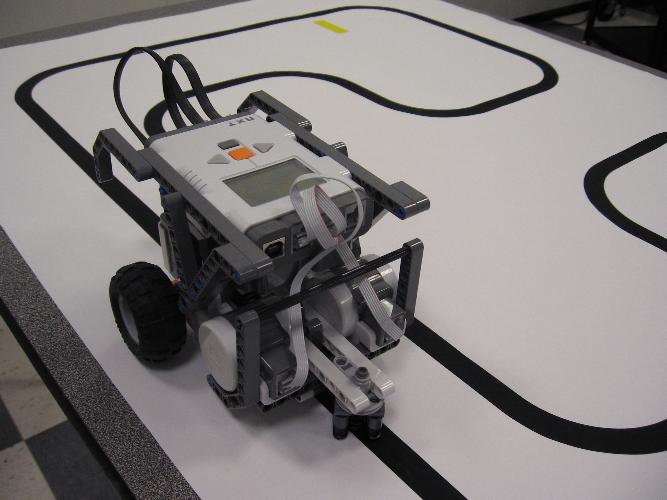
\includegraphics[width = \linewidth]{Abstract/Black-line-in-white-area.jpg}
						\caption{Black line}
						\label{subfiger:A}
					\end{subfigure}
					
					\vspace{5mm}
	
					\begin{subfigure}[normal]{0.3\textwidth}
						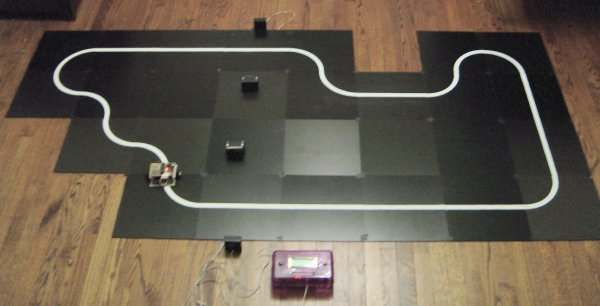
\includegraphics[width = \linewidth]{Abstract/white-line-in-black-area.jpg}
						\caption{white line}
						\label{subfiger:B}
					\end{subfigure}
					\caption{Different area - Line Follow}
					
			\end{center}	
		\end{figure}
	\end{abstract}

	\pagenumbering{roman}
	\newpage
	\tableofcontents
		
	
	\newpage
	\pagenumbering{arabic}
	
	
	\newpage
	\chapter{ Introduction}
		\begin{figure}[H]
			\begin{center}
				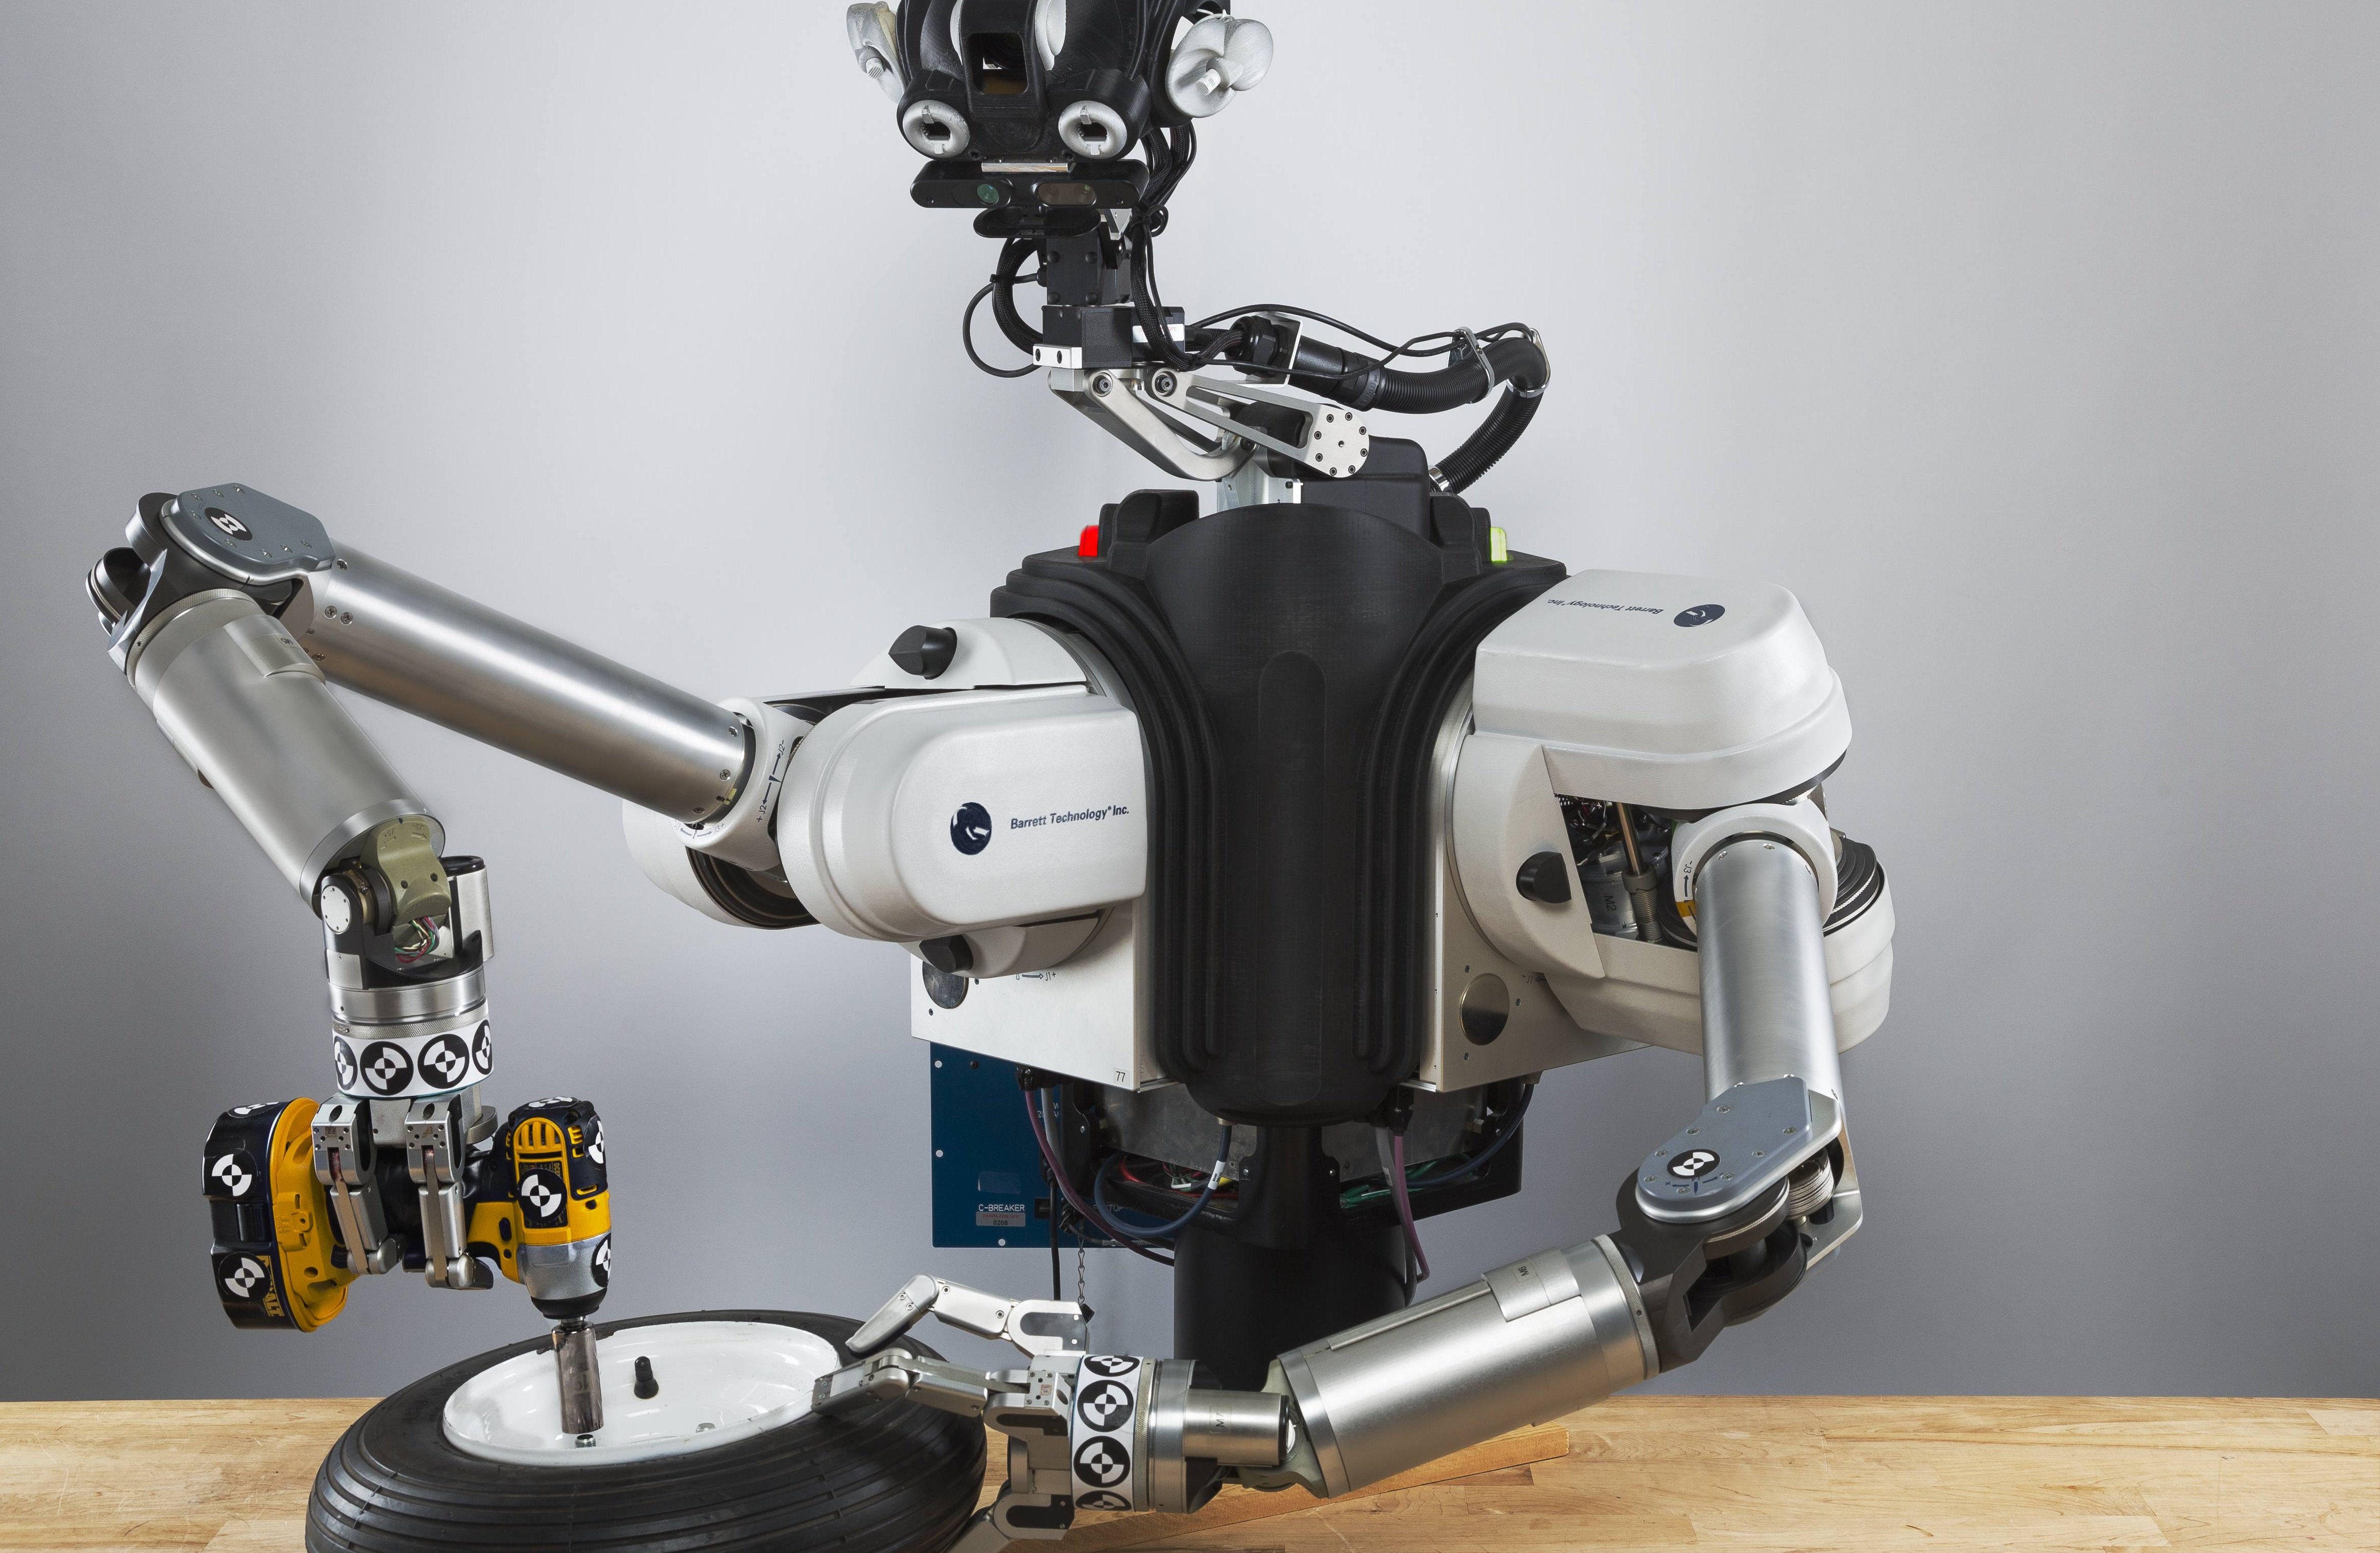
\includegraphics[scale = 0.19]{Ch1-Introduction/Multi-Degree-Robot.jpg}
				\caption{Multi-Degree-Robot}
				\label{fig:Multi-Degree-Robot}
			\end{center}
		\end{figure}
		An autonomous robot is a robot that performs behaviors or tasks with a high degree of autonomy, which is particularly desirable in fields such as spaceflight, household maintenance (such as cleaning), waste water treatment and delivering goods and services.
		
		Some modern factory robots are "autonomous" within the strict confines of their direct environment. It may not be that every degree of freedom exists in their surrounding environment, but the factory robot's workplace is challenging and can often contain chaotic, unpredicted variables. The exact orientation and position of the next object of work and (in the more advanced factories) even the type of object and the required task must be determined. This can vary unpredictably (at least from the robot's point of view).

		One important area of robotics research is to enable the robot to cope with its environment whether this be on land, underwater, in the air, underground, or in space.
		\\ \\ \\ \\ \\
///		A fully autonomous robot can:\\
			1-Gain information about the environment.\\
			2-Work for an extended period without human intervention.\\
			3-Move either all or part of itself throughout its operating environment without human assistance.\\
			4-Avoid situations that are harmful to people, property, or itself unless those are part of its design specifications.\\
			
			An autonomous robot may also learn or gain new knowledge like adjusting for new methods of accomplishing its tasks or adapting to changing surroundings.

		Like other machines, autonomous robots still require regular maintenance.\\ \\
// cet here here $https://en.wikipedia.org/wiki/Autonomous_robot$
	
	\newpage
	\chapter{Planning }
		\begin{figure}[ht]
			\begin{center}
				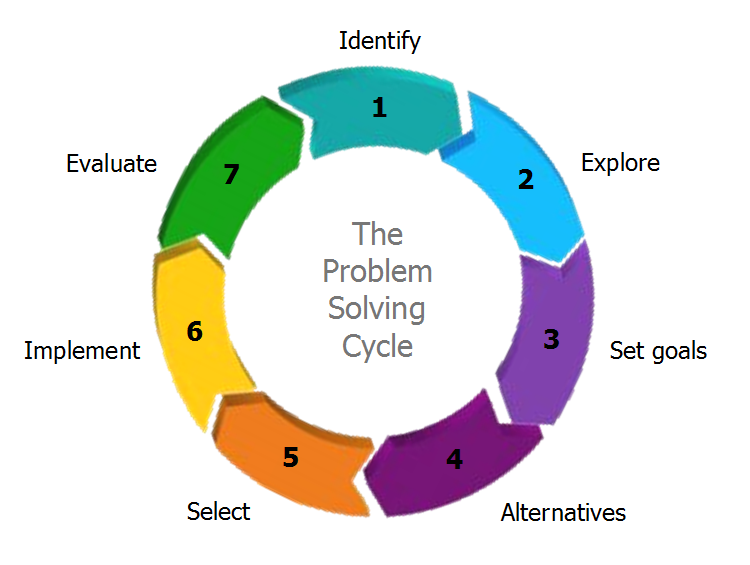
\includegraphics[scale=0.3]{Ch2-Planning/Problem-Solving-Steps}
				\caption{Problem-Solving-Steps}
				%\lable{}
			\end{center}
		\end{figure}
		
		
		\section{\textbf{Identify}}
		At the begining we got an identifying mission from the instructor " Ahmed Abdelbasit " \begin{quotation}
  				\begin{figure}[ht]
					\begin{center}
						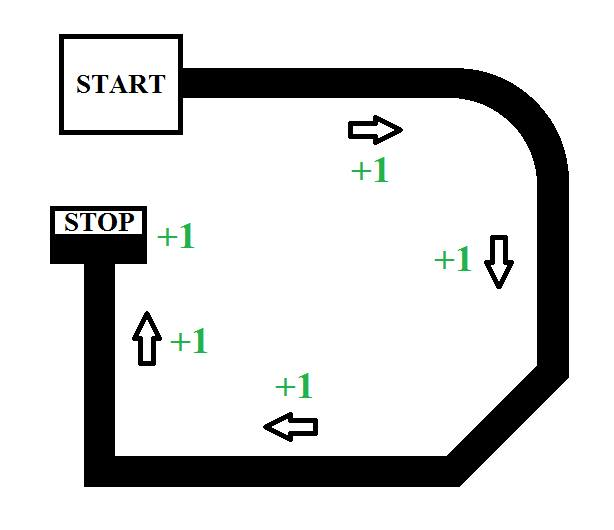
\includegraphics[scale=0.2]{Ch2-Planning/Idenfying-Mission}
						\caption{Idenfying-Mission}
						%\lable{}
					\end{center}
			\end{figure}
			
				1- Our 3rd mini project is to make a line follower robot able to pass through the track shown in the attached photo. 
				
				2-The track is divided into 5 check points each increases your grade by a single point.
				
				3-Our track line width is 4 cm.
				
				4-Your robot must stop automatically at the last check point.
				
				5-You must design and fabricate a creative robot chassis using maximum 2 sheets of wood. 
				
				6-Documentation must be written in Latex, follow the technical report layout we discussed and delivered in pdf file format. 
				
				7-Due date is next Monday 18/9/2017 
				
			\end{quotation}
			
		\section{\textbf{Explore	}} 
		 
		The mission was clear enouf for us , so we start sarshing on the internet web sites to collect more information about "Line Follower Robot" , watching videos of working ones to notice other mistakes to avoid them and reading different codes.
		We ended with a good conception about what we have to do , then we moved to what we missid and what we do not know about  our resorces in our "Mini-Fab-Lab".
		
		\newpage
		\section{\textbf{Set Goals}}  
		
		We found some amazing projects and some other insignificant , but we was restricted by our limited time and resorces , so our goals :
		
		1-Use minimum components
		
		2-Write an efficient orginzed code
		
		3-Build a butiful car model
		
		4-Write a good profitional documentation
		
		5-Make a good  presentation
		
		and nice to have :
		
		6-Make a PCB instead of using bread-board
		
		\newpage 
		\section{\textbf{Components and Alternatives}} 
		
		The component we choosed ware:
		
		-Two continouse DC motors 
		
		-Two wheels (10cm diam)
		
		-One Caster-Ball
		
		-One L293D H-Bridge IC
		
		-Arduino uno kit.
		
		
		The Alternatives ware to choose between:
		
		-Two IR-Sensors VS Two LDR-Sensors
		
		we choosed IR-Sensors , because it adjustable.
		
		\begin{figure}[H]
			\begin{center}
					\begin{subfigure}[normal]{0.4\textwidth}
						\includegraphics[scale=0.1]{From-Mobile/Some-Components.jpg}
						\caption{Diff-Components}
						\label{subfiger:A}
						
						%\vspace{5mm}
						
						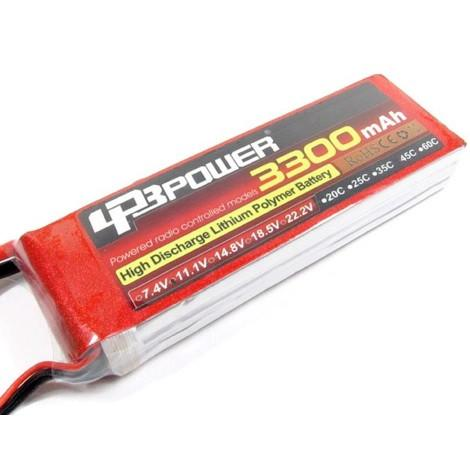
\includegraphics[scale=0.1]{Ch2-Planning/Lithuime-Bettary.jpg}
						\caption{Lithuime-Bettary}
						\label{subfiger:B}
						
						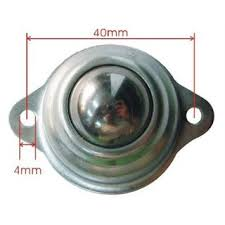
\includegraphics[scale=0.2]{Ch2-Planning/Caster-Ball.jpg}
						\caption{Caster-Ball}
						\label{subfiger:c}
						
						
					\end{subfigure}
					\caption{Components}
			\end{center}	
		\end{figure}
		

	
	\newpage
	\chapter{Learning} 
	Thought and planing is just the beginning.First of all we start to analyze and devide the project into pecies , software and hardware.Figure 3.2
	
	At software part we build a small circuit by H-bridge to test the motors and sensros to make sure it works.Then we connect the arduino and wrote a simple code to choose a sutable speed of motors which modify later in trial model.
	
	From the other side at the hardware , there was available an olde model its design was near to our design and we were allowed to try the road three times , so we used in it experimental try to test the software and to avoid hardware mistakes that may meet us.
	\begin{figure}[h]
					\begin{center}
						\includegraphics[scale=0.1]{Ch2-Planning/Experimental-Try}
						\caption{Experimental-Try}
						%\lable{}
					\end{center}
	\end{figure}
	
	\begin{figure}[b]
					\begin{center}
						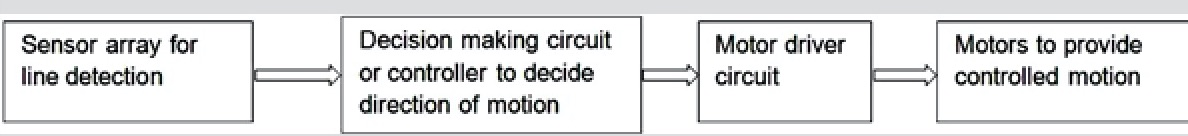
\includegraphics[scale=0.2]{Ch2-Planning/Block-Diag}
						\caption{Analyzing}
						%\lable{fig:fig3.1}
					\end{center}
	\end{figure}
	
	
	\newpage
	\chapter{Executing}
	
	\section{Electric and Software}
	
		Building a Semi-Final Circuit via a bread-board and other components.Figure 4.1 
		
		Then write a sutabale code Figure 4.2, after that we tested that code Fig4.3 (a) , we recogize the field reason which was the sensor placed from the motors and its installation Fig4.3 (b) and fixed it temporarily and keeped in mind in design stage.
		
		
		
		
		\begin{figure}[b]
			\begin{center}
				%\includegraphics[scale=0.1]{Ch4-Executing/Experimental-Try}
				\caption{Semi-Final Circuit}
				%\lable{}
			\end{center}
		\end{figure}
		
		\begin{figure}[]
			
					\begin{subfigure}[normal]{0.5\textwidth}
						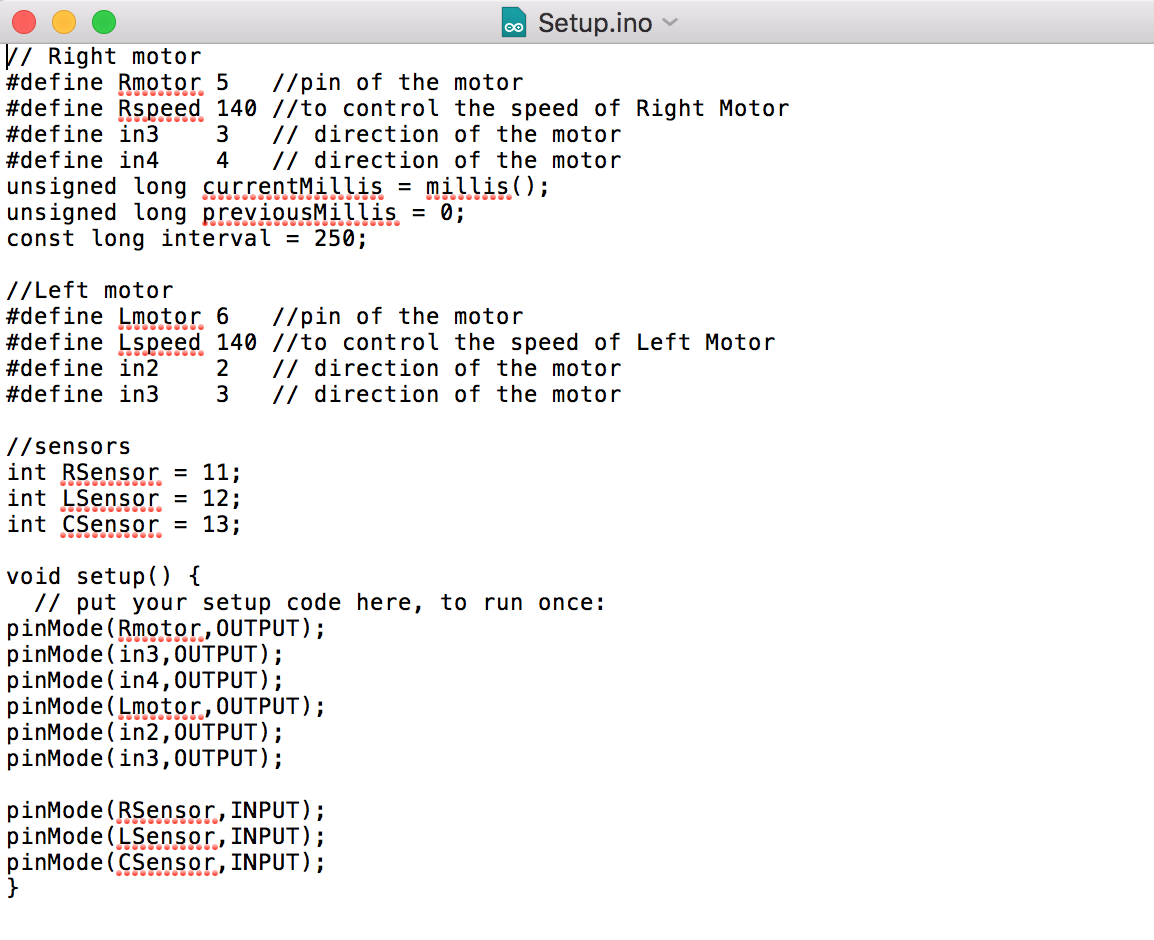
\includegraphics[scale=0.3]{Ch4-Executing/Code-Setup-Part}
						\caption{Code-Setup-Part}
						\label{subfiger:A}
												
						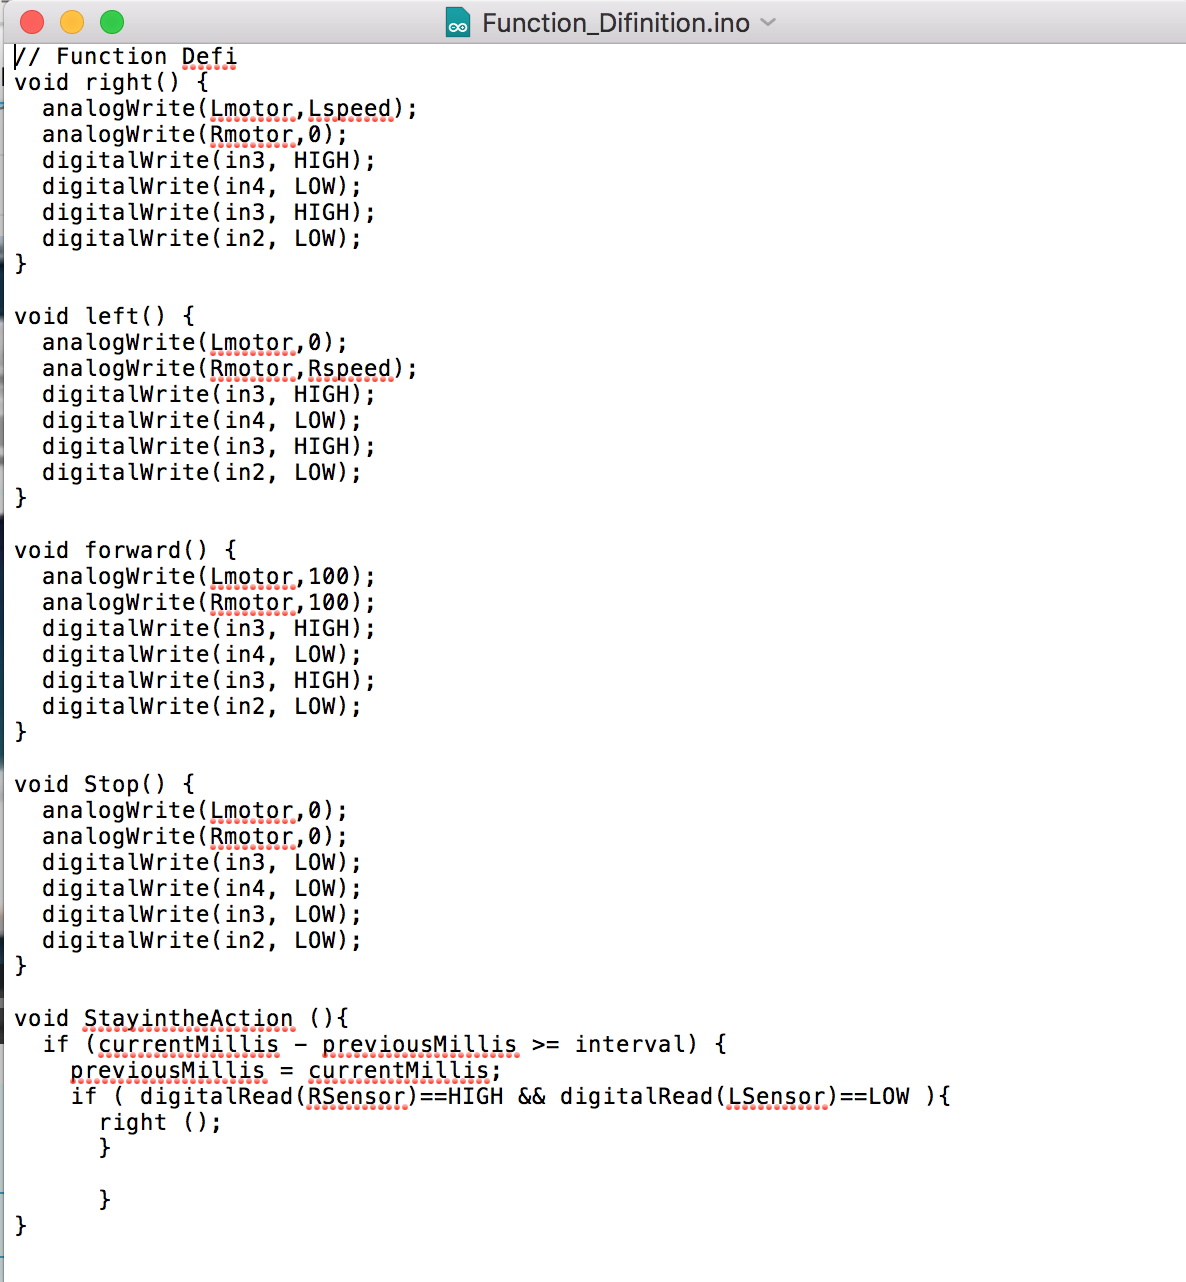
\includegraphics[scale=0.3]{Ch4-Executing/Code-Fun_Diff-Part}
						\caption{Code-Fun-Diff-Part}
						\label{subfiger:B}
						
						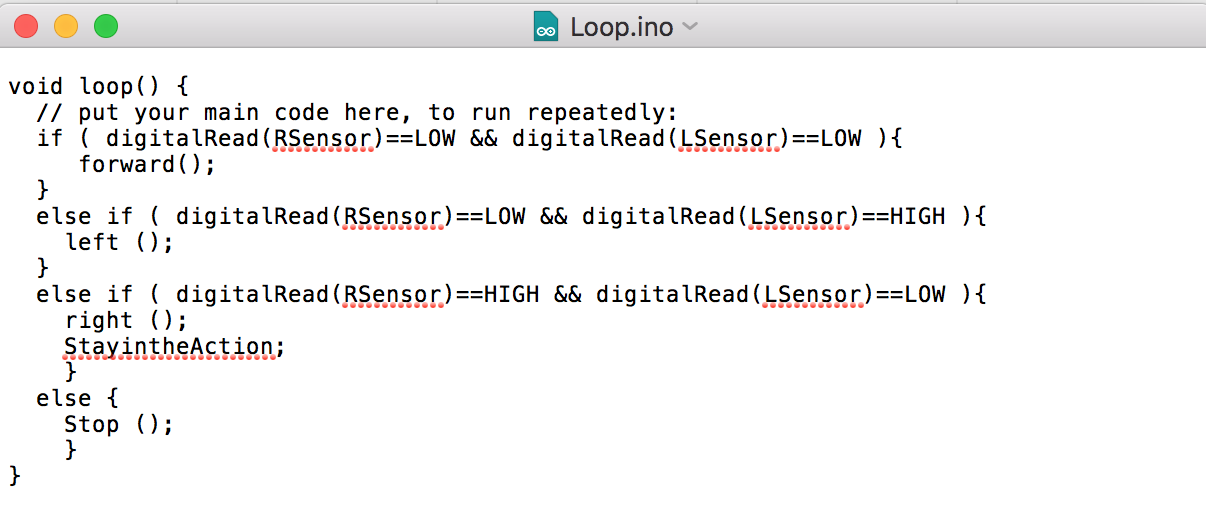
\includegraphics[scale=0.3]{Ch4-Executing/Code-Loop-Part}
						\caption{Code-Loop-Part}
						\label{subfiger:c}
						
						
					\end{subfigure}
					\caption{Code Components}
			
		\end{figure}
		
		\begin{figure}[ht]
			%\end{center}
				\begin{subfigure}[normal]{0.5\textwidth}
					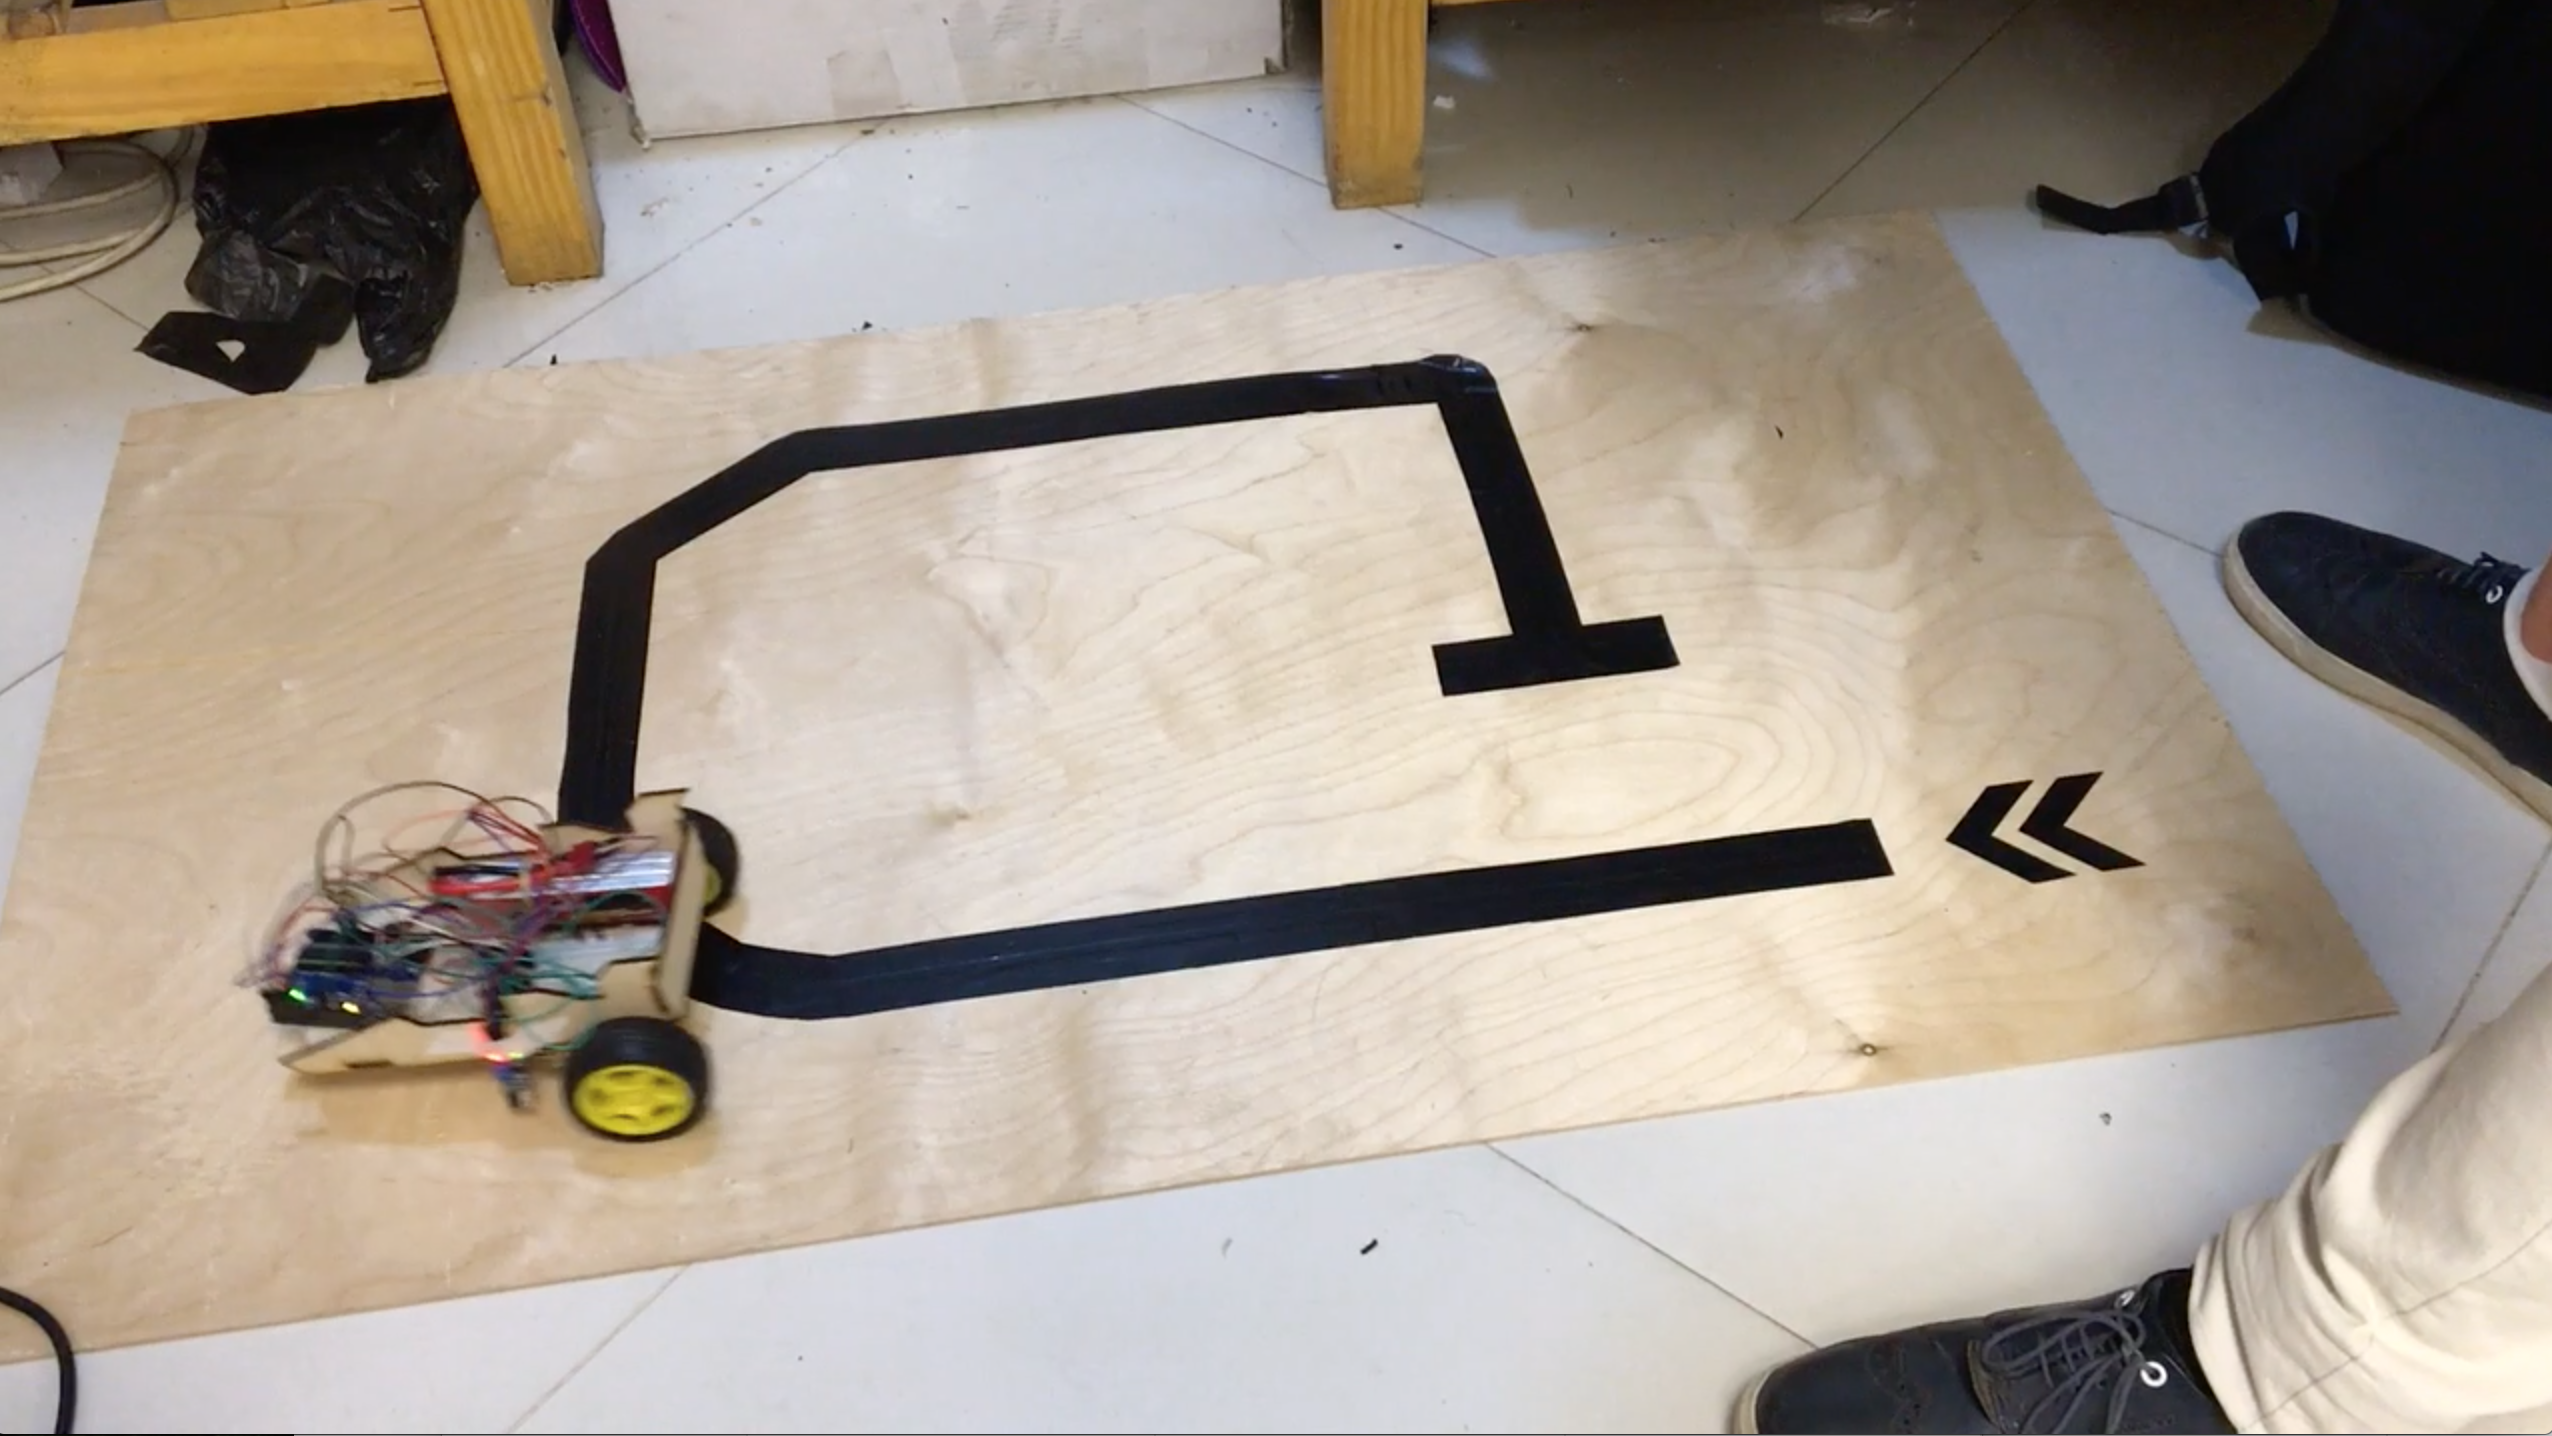
\includegraphics[scale=0.15]{Ch4-Executing/Experiment-Try-One}
					\caption{Experiment-Try-Failed-One}
					\label{A}
			
					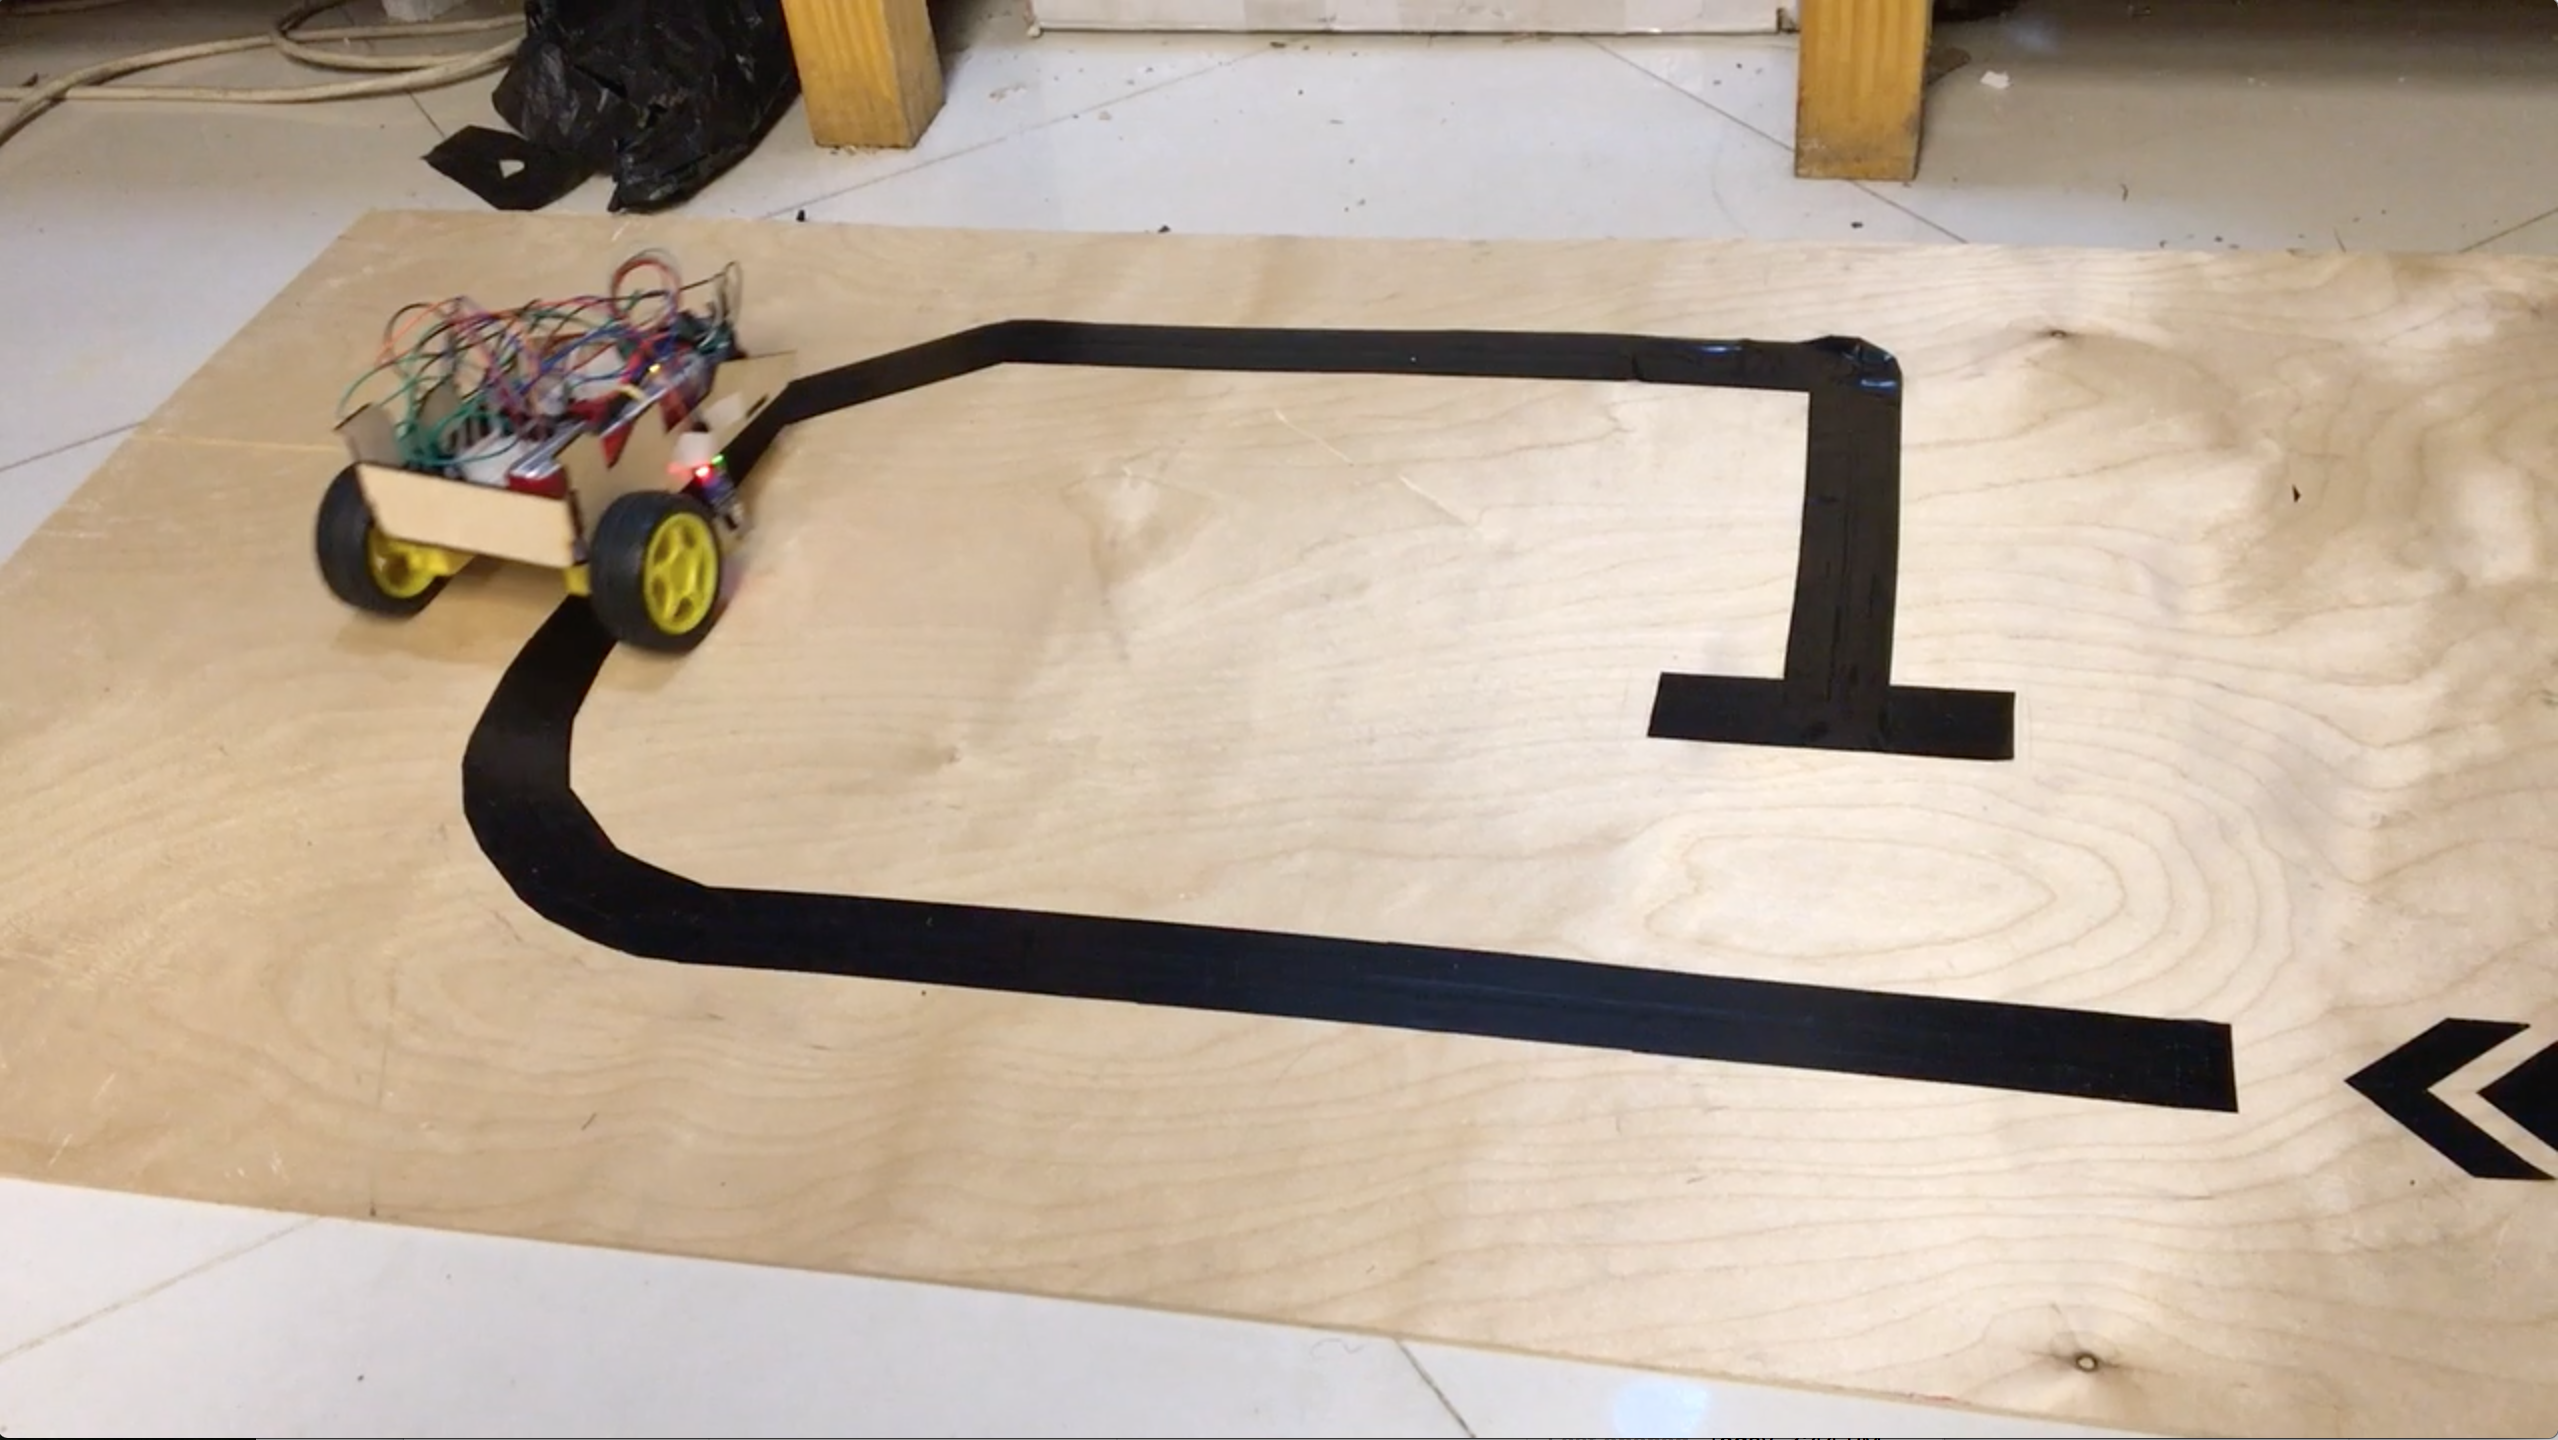
\includegraphics[scale=0.15]{Ch4-Executing/Experiment-Try-Two}
					\caption{Experiment-Try-Sucsses-Two}
					\label{B}
					
				\end{subfigure}
				\caption{Experiments}
			%\end{center}
		\end{figure}
	\newpage
	\newpage
	\newpage
	\newpage
	\section{Mechanics and Hardware}
	
		We designed the care body on SolidWorks ,  then assembeled the to insure it is fine , finally saved it as .dfx Figure .
		
		After that we moved to Laser cutter and used "moshi" prog to control the machine.
		
		\begin{figure}[]
			\begin{center}
				\begin{subfigure}[normal]{0.5\textwidth}
					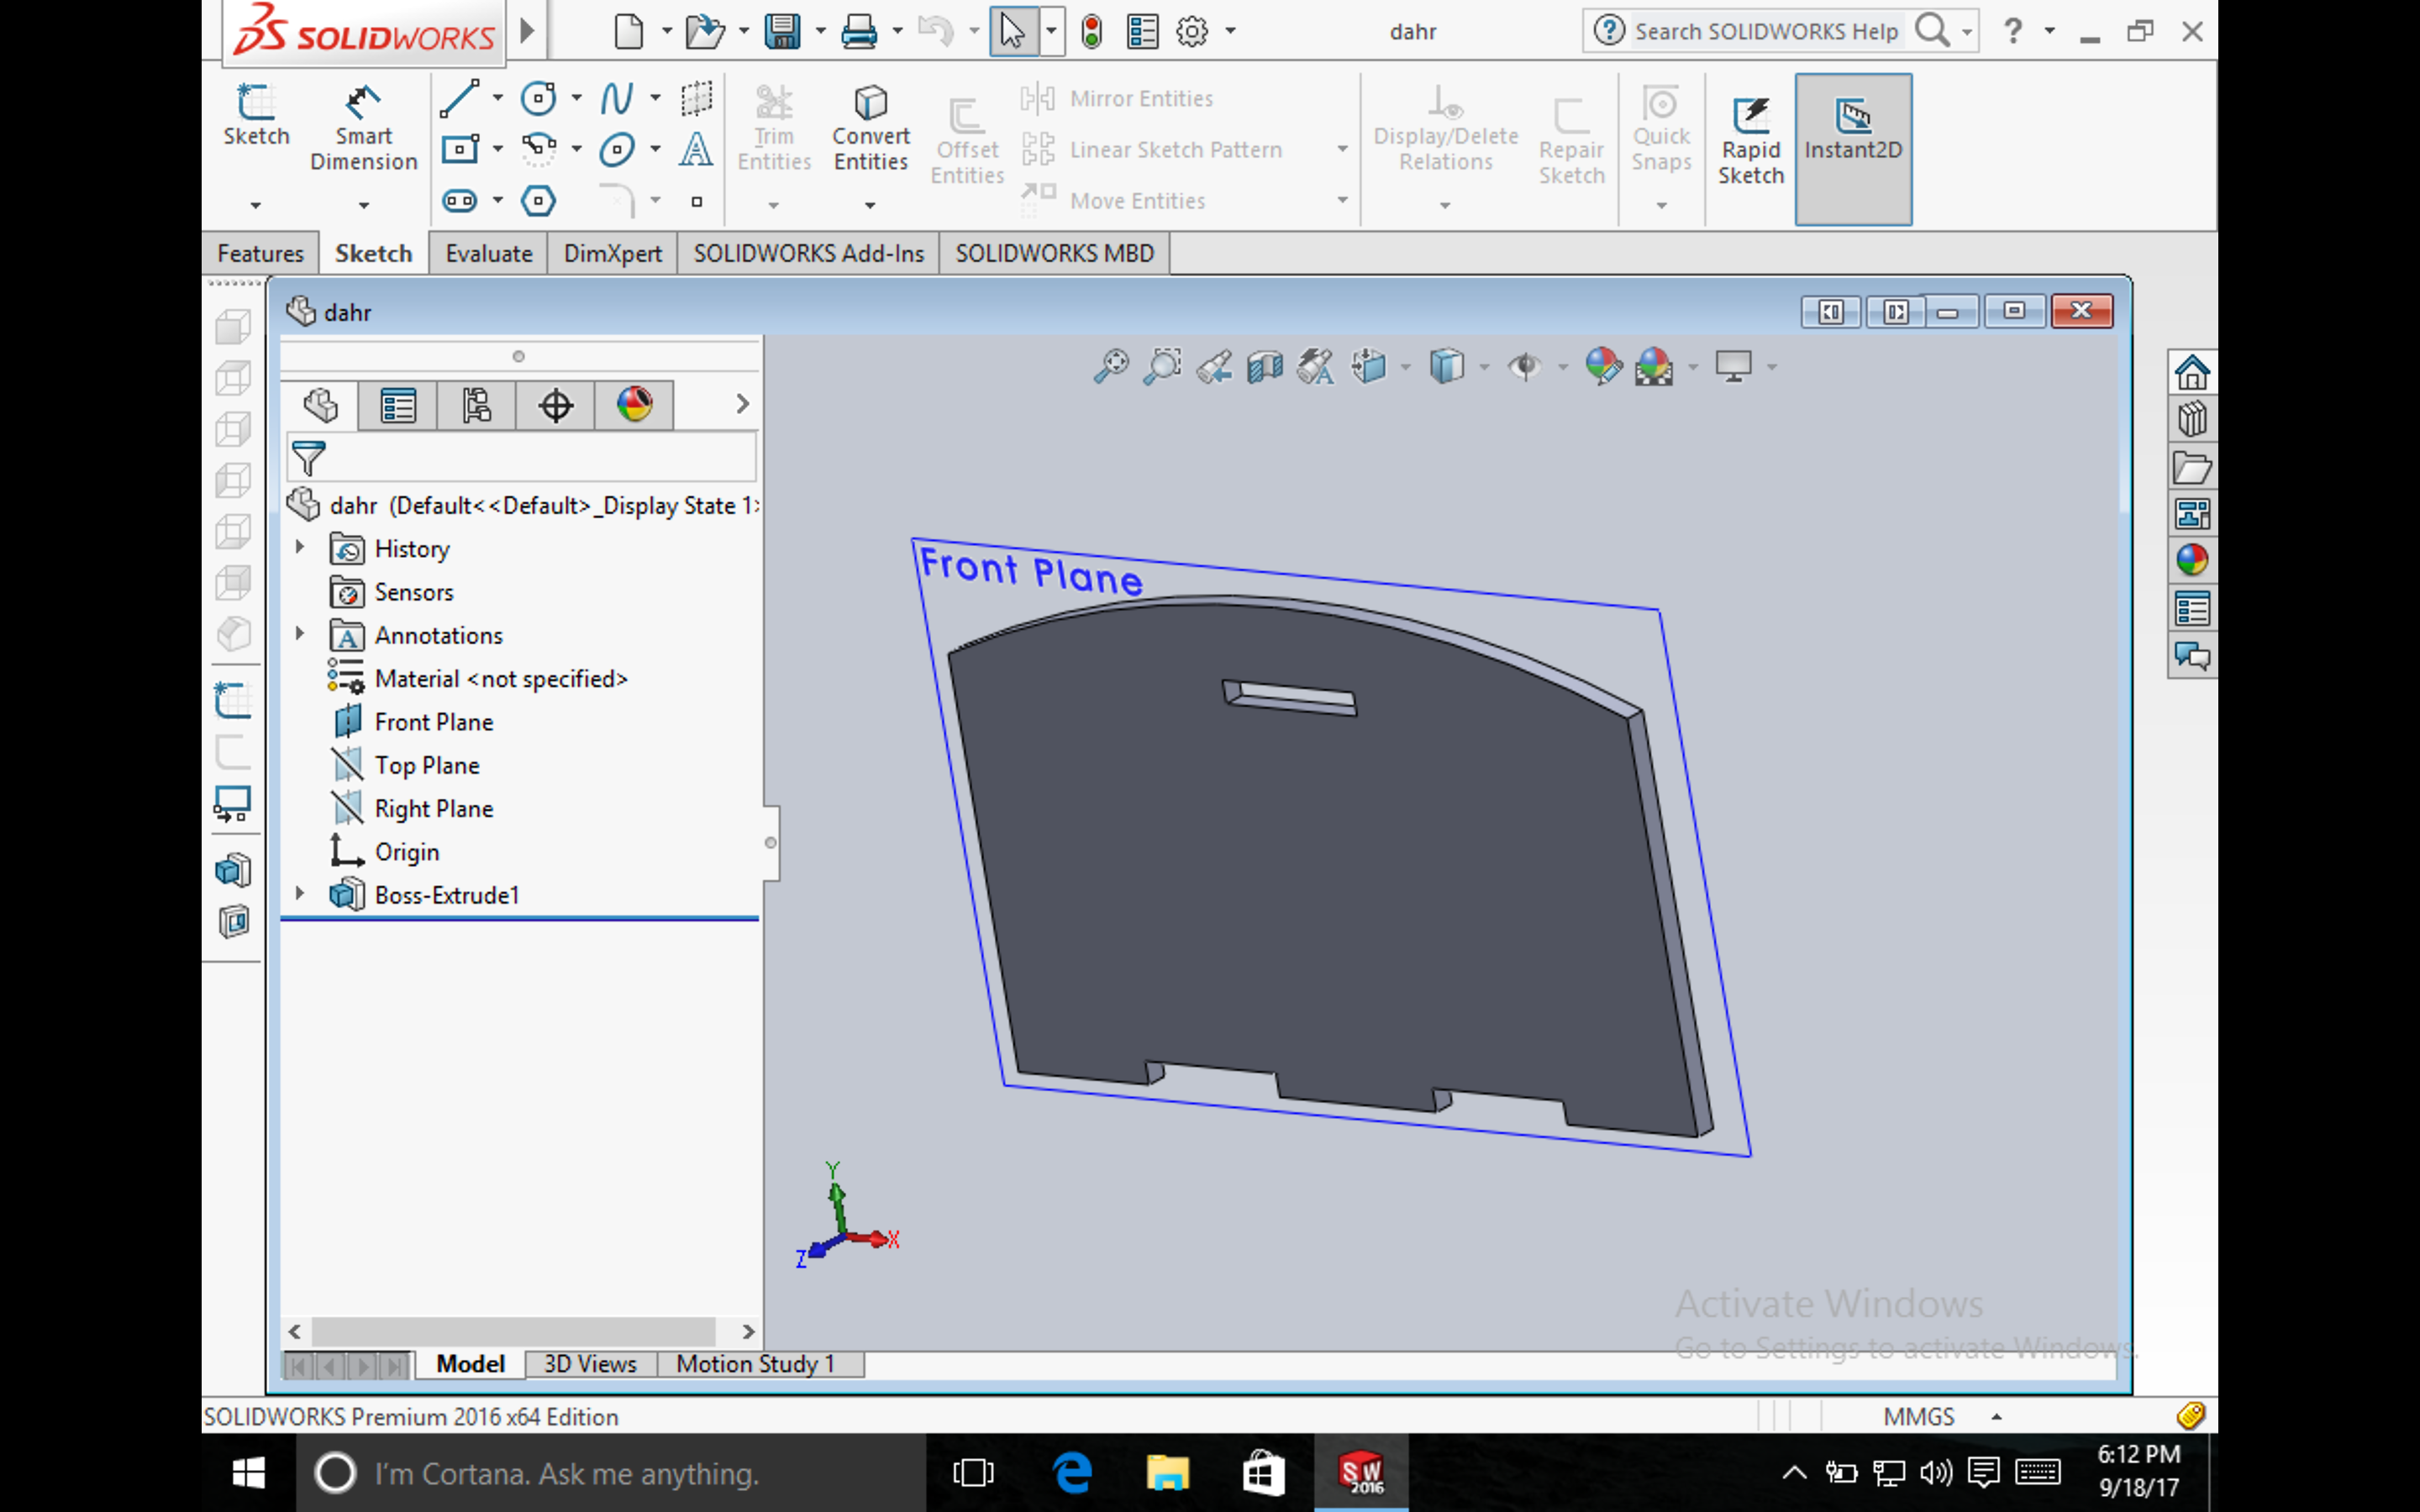
\includegraphics[scale=0.13]{Ch4-Executing/Mechanical-Desin-SolidWorks}
					\caption{}
					\label{A}
					
					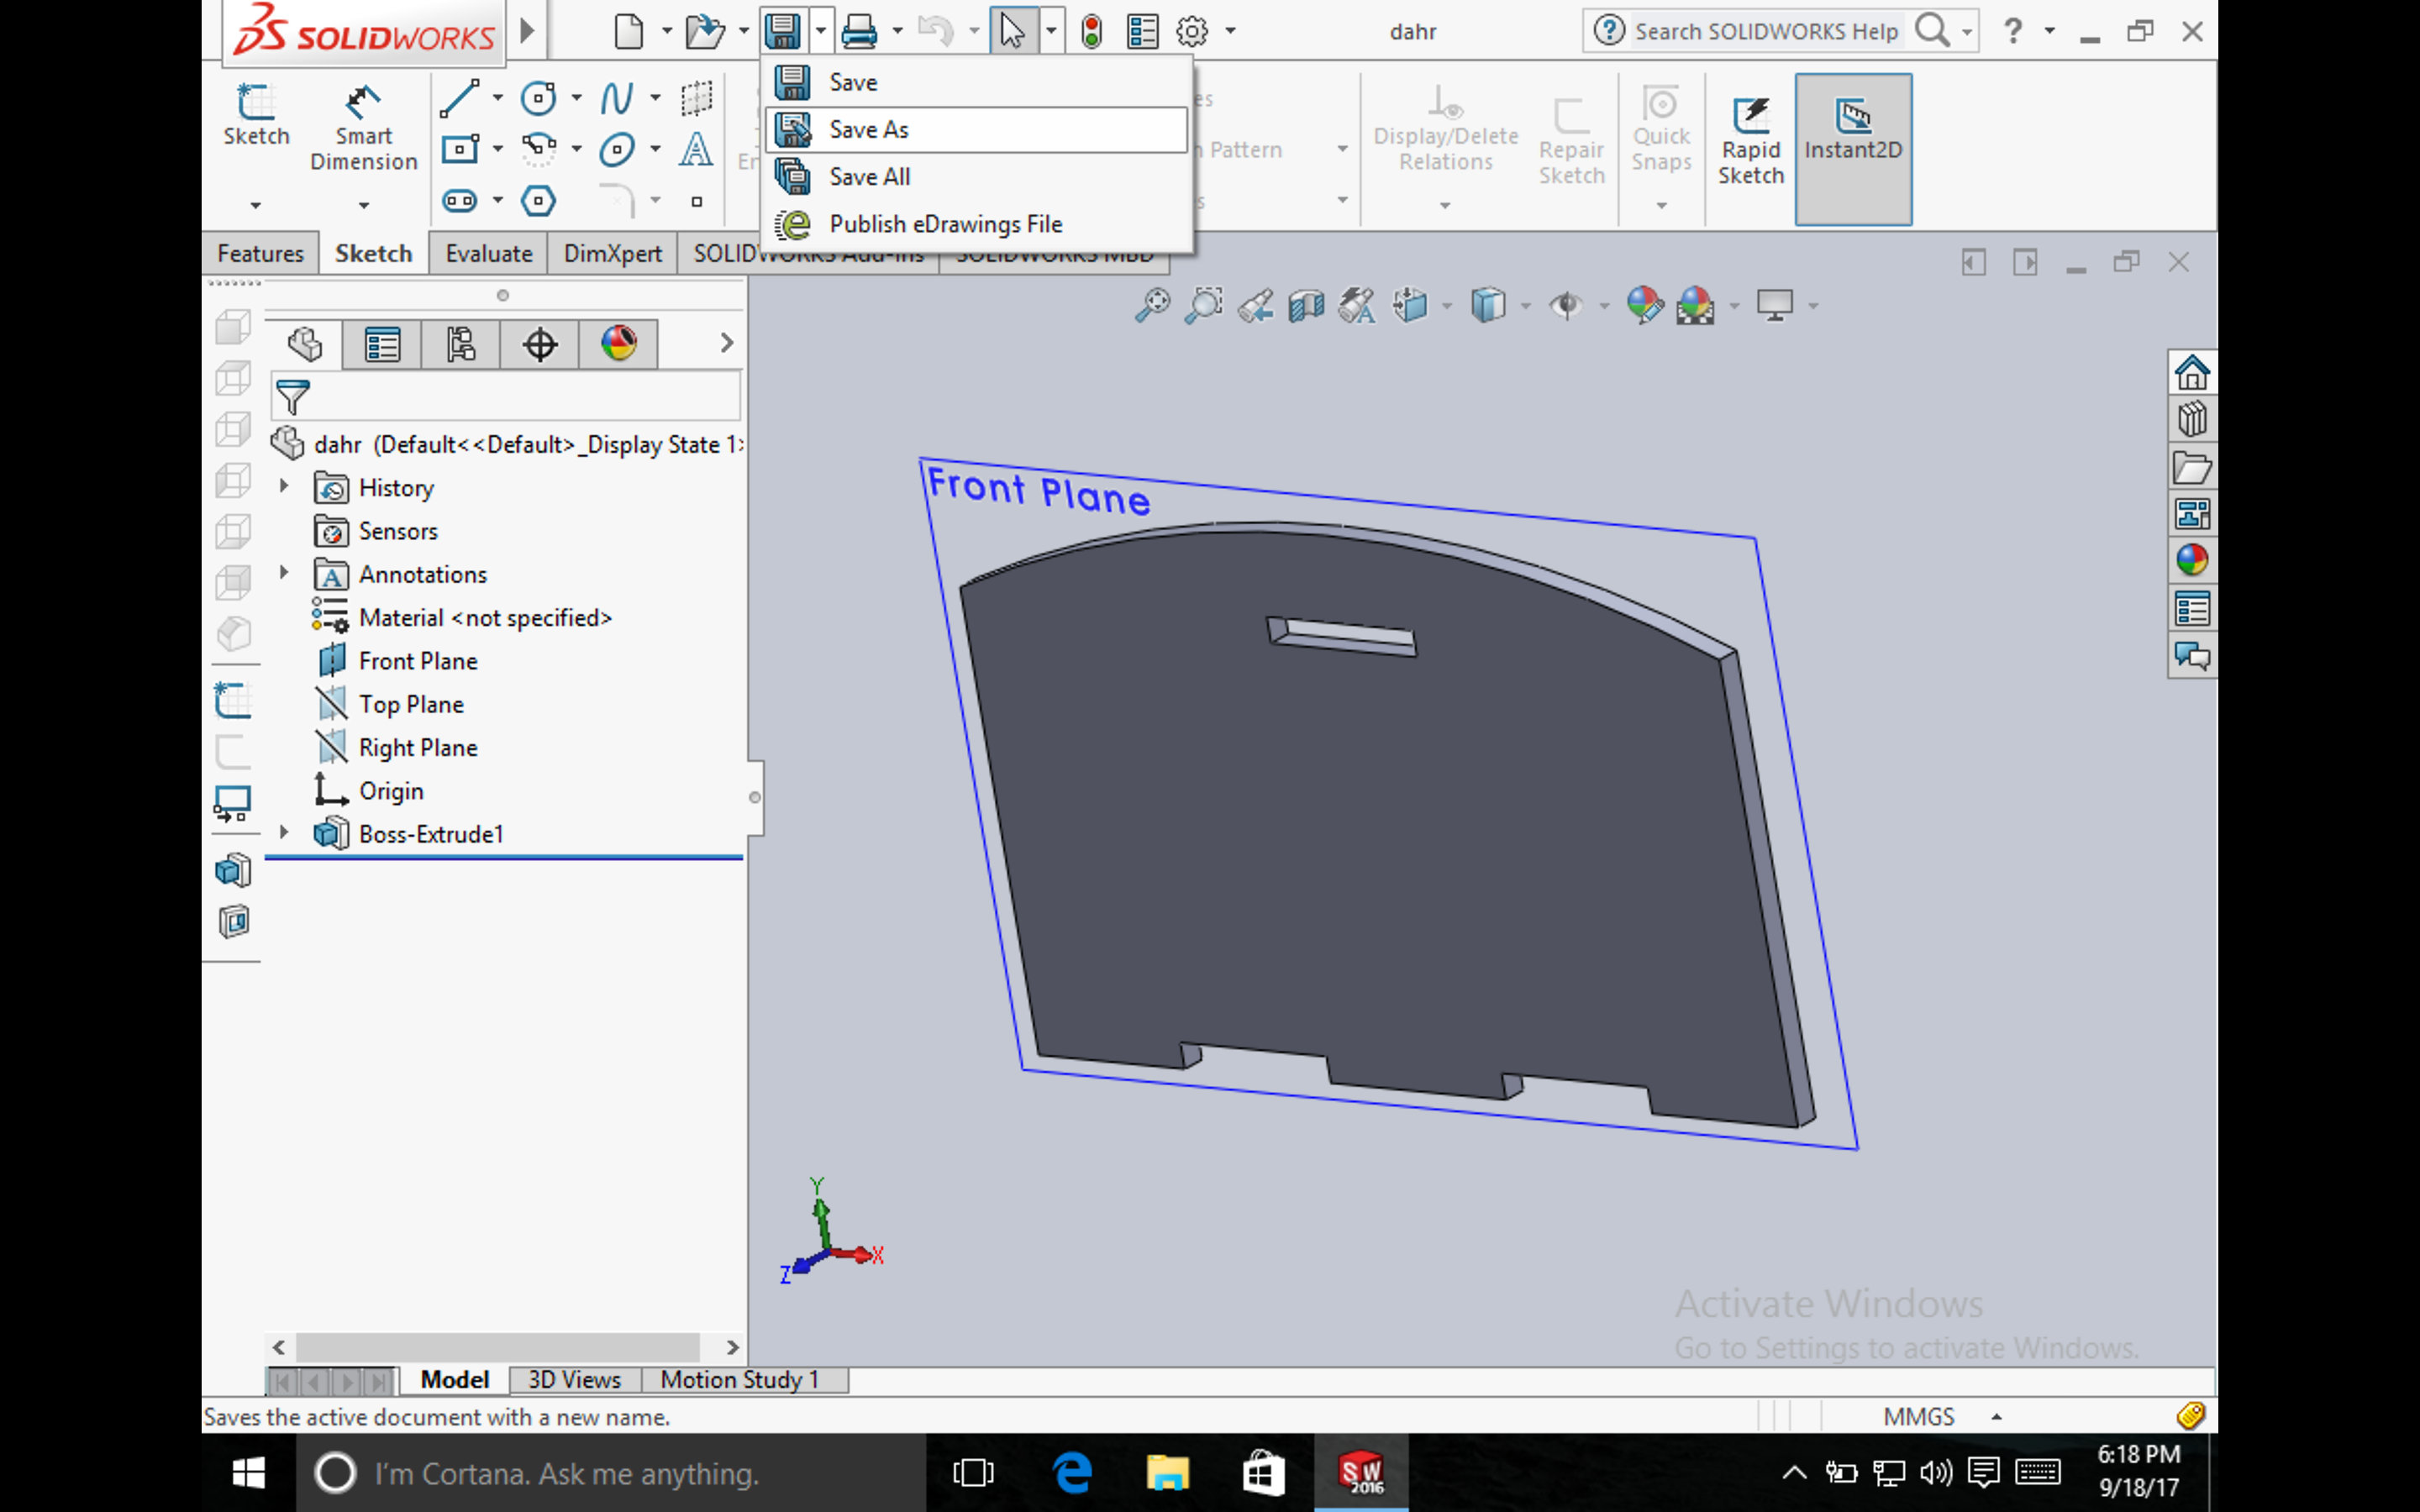
\includegraphics[scale=0.12]{Ch4-Executing/1}
					\caption{}
					\label{B}
			
					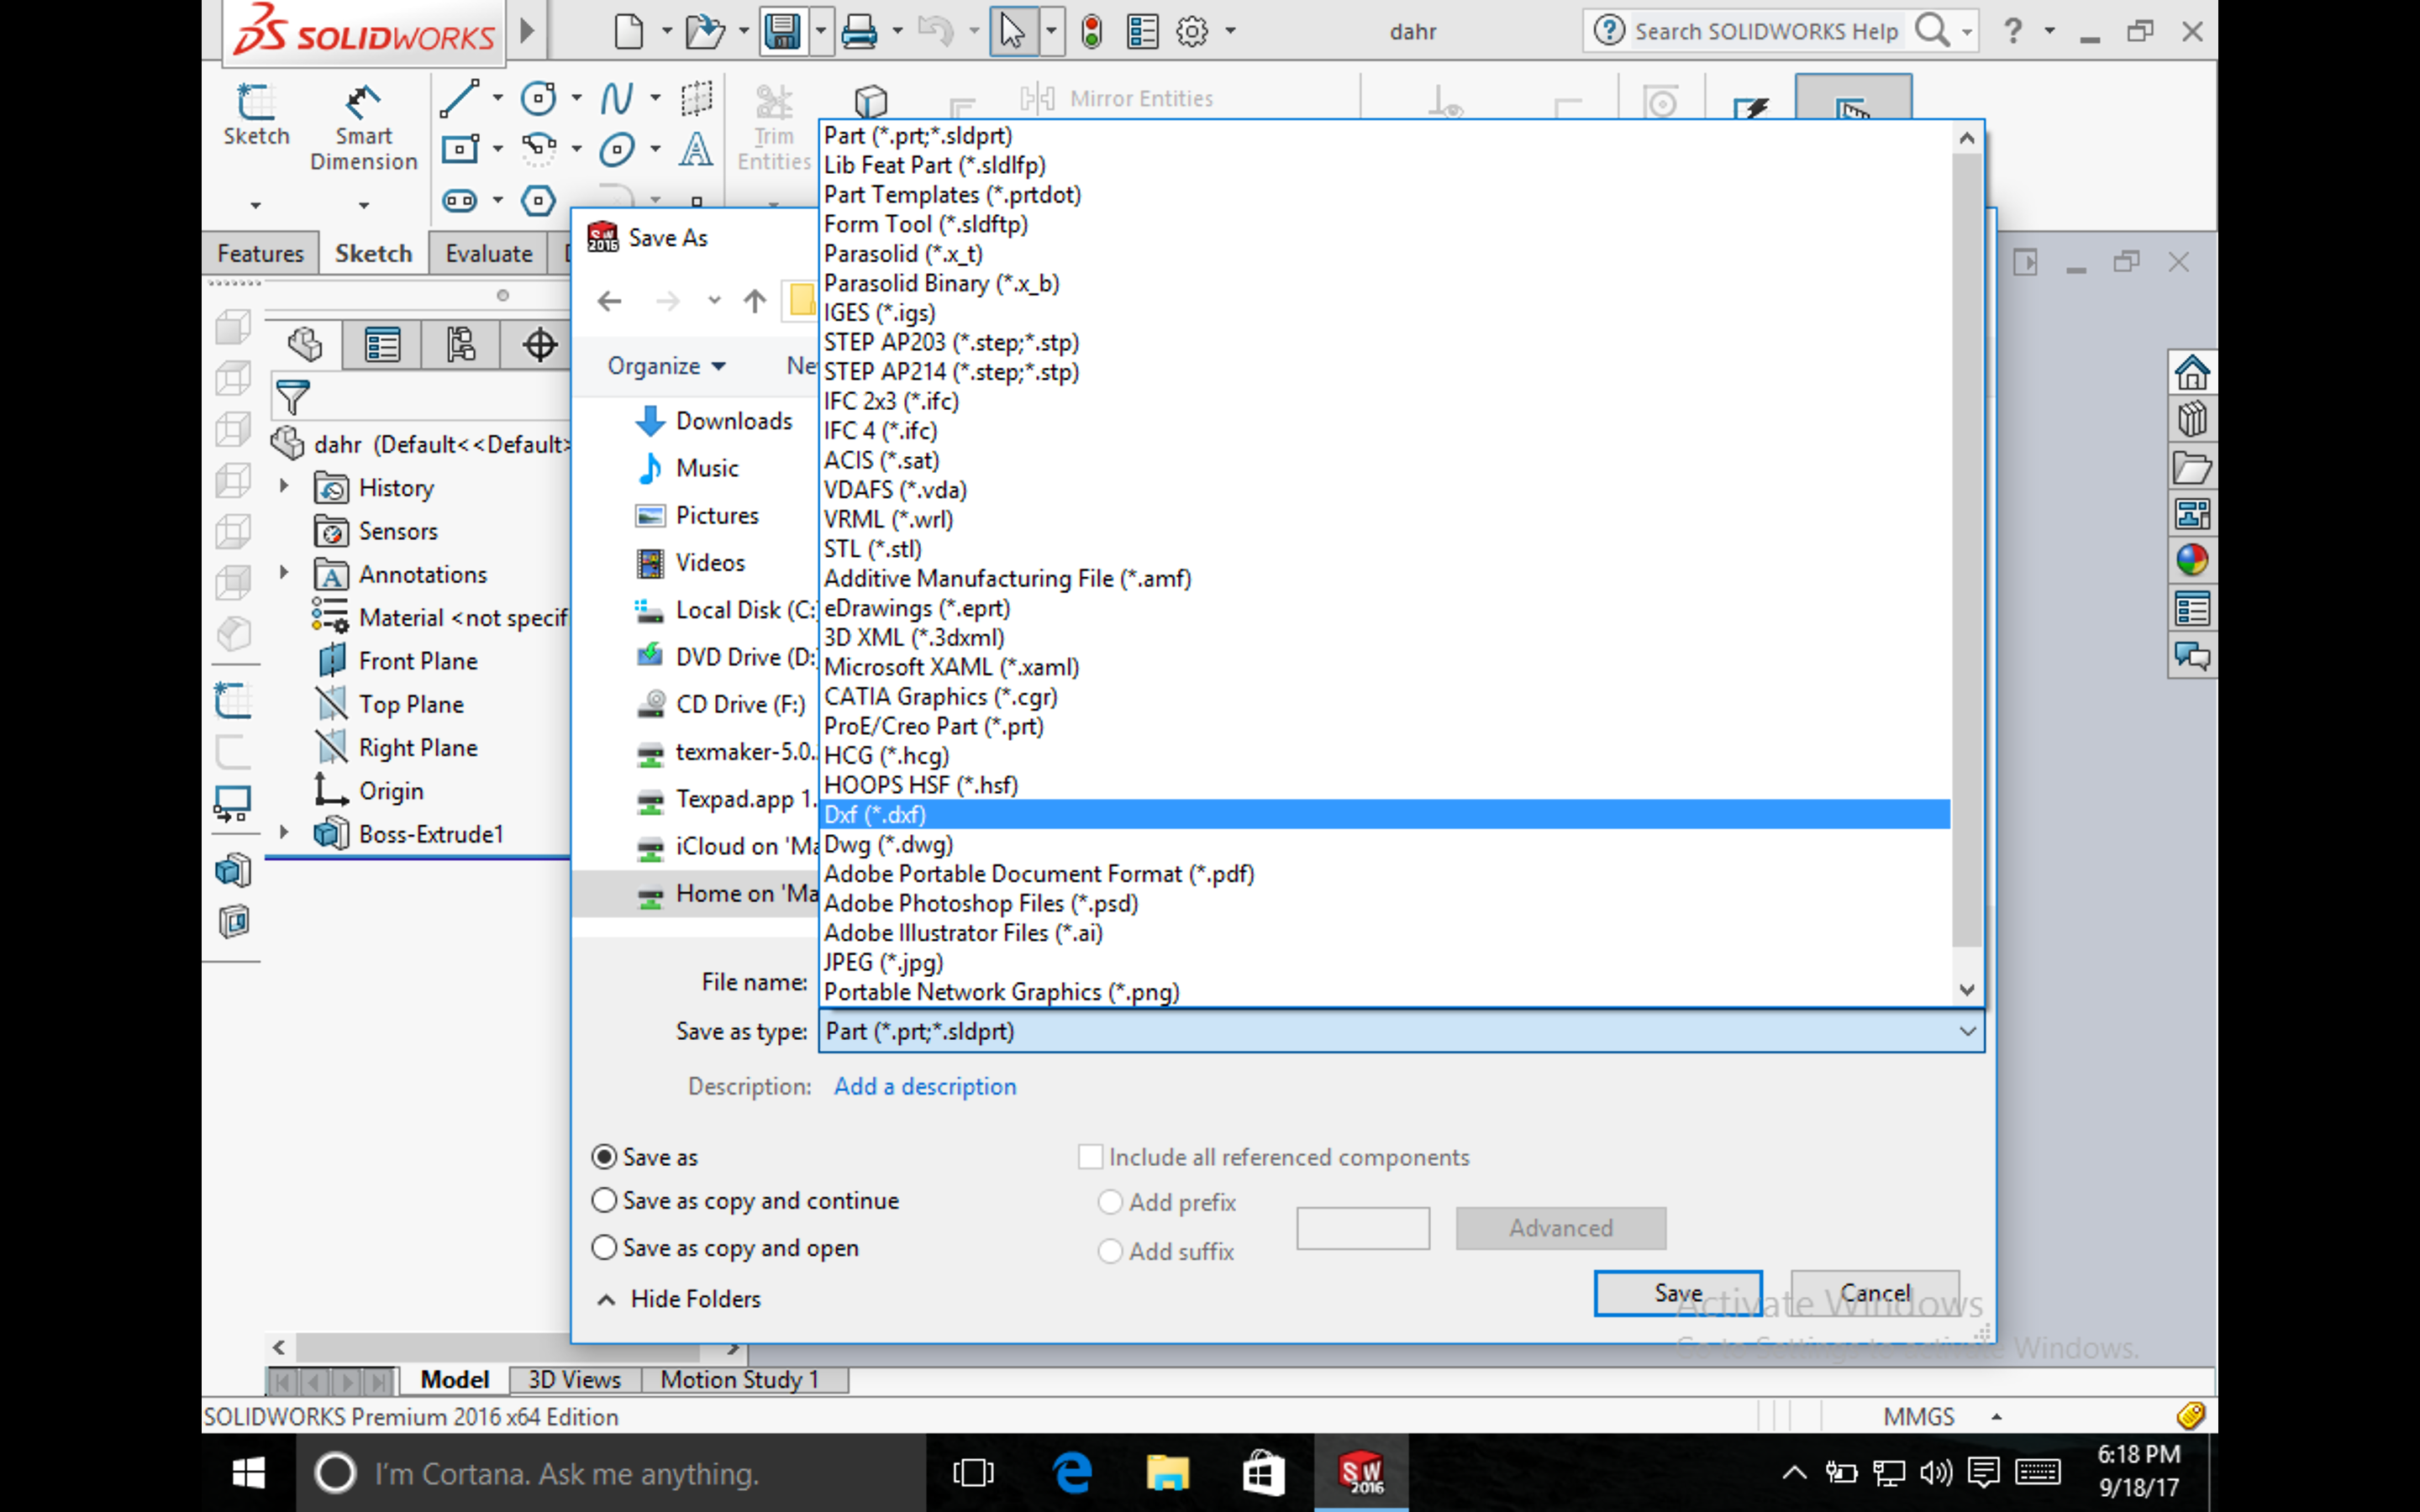
\includegraphics[scale=0.12]{Ch4-Executing/2}
					\caption{}
					\label{C}
					
					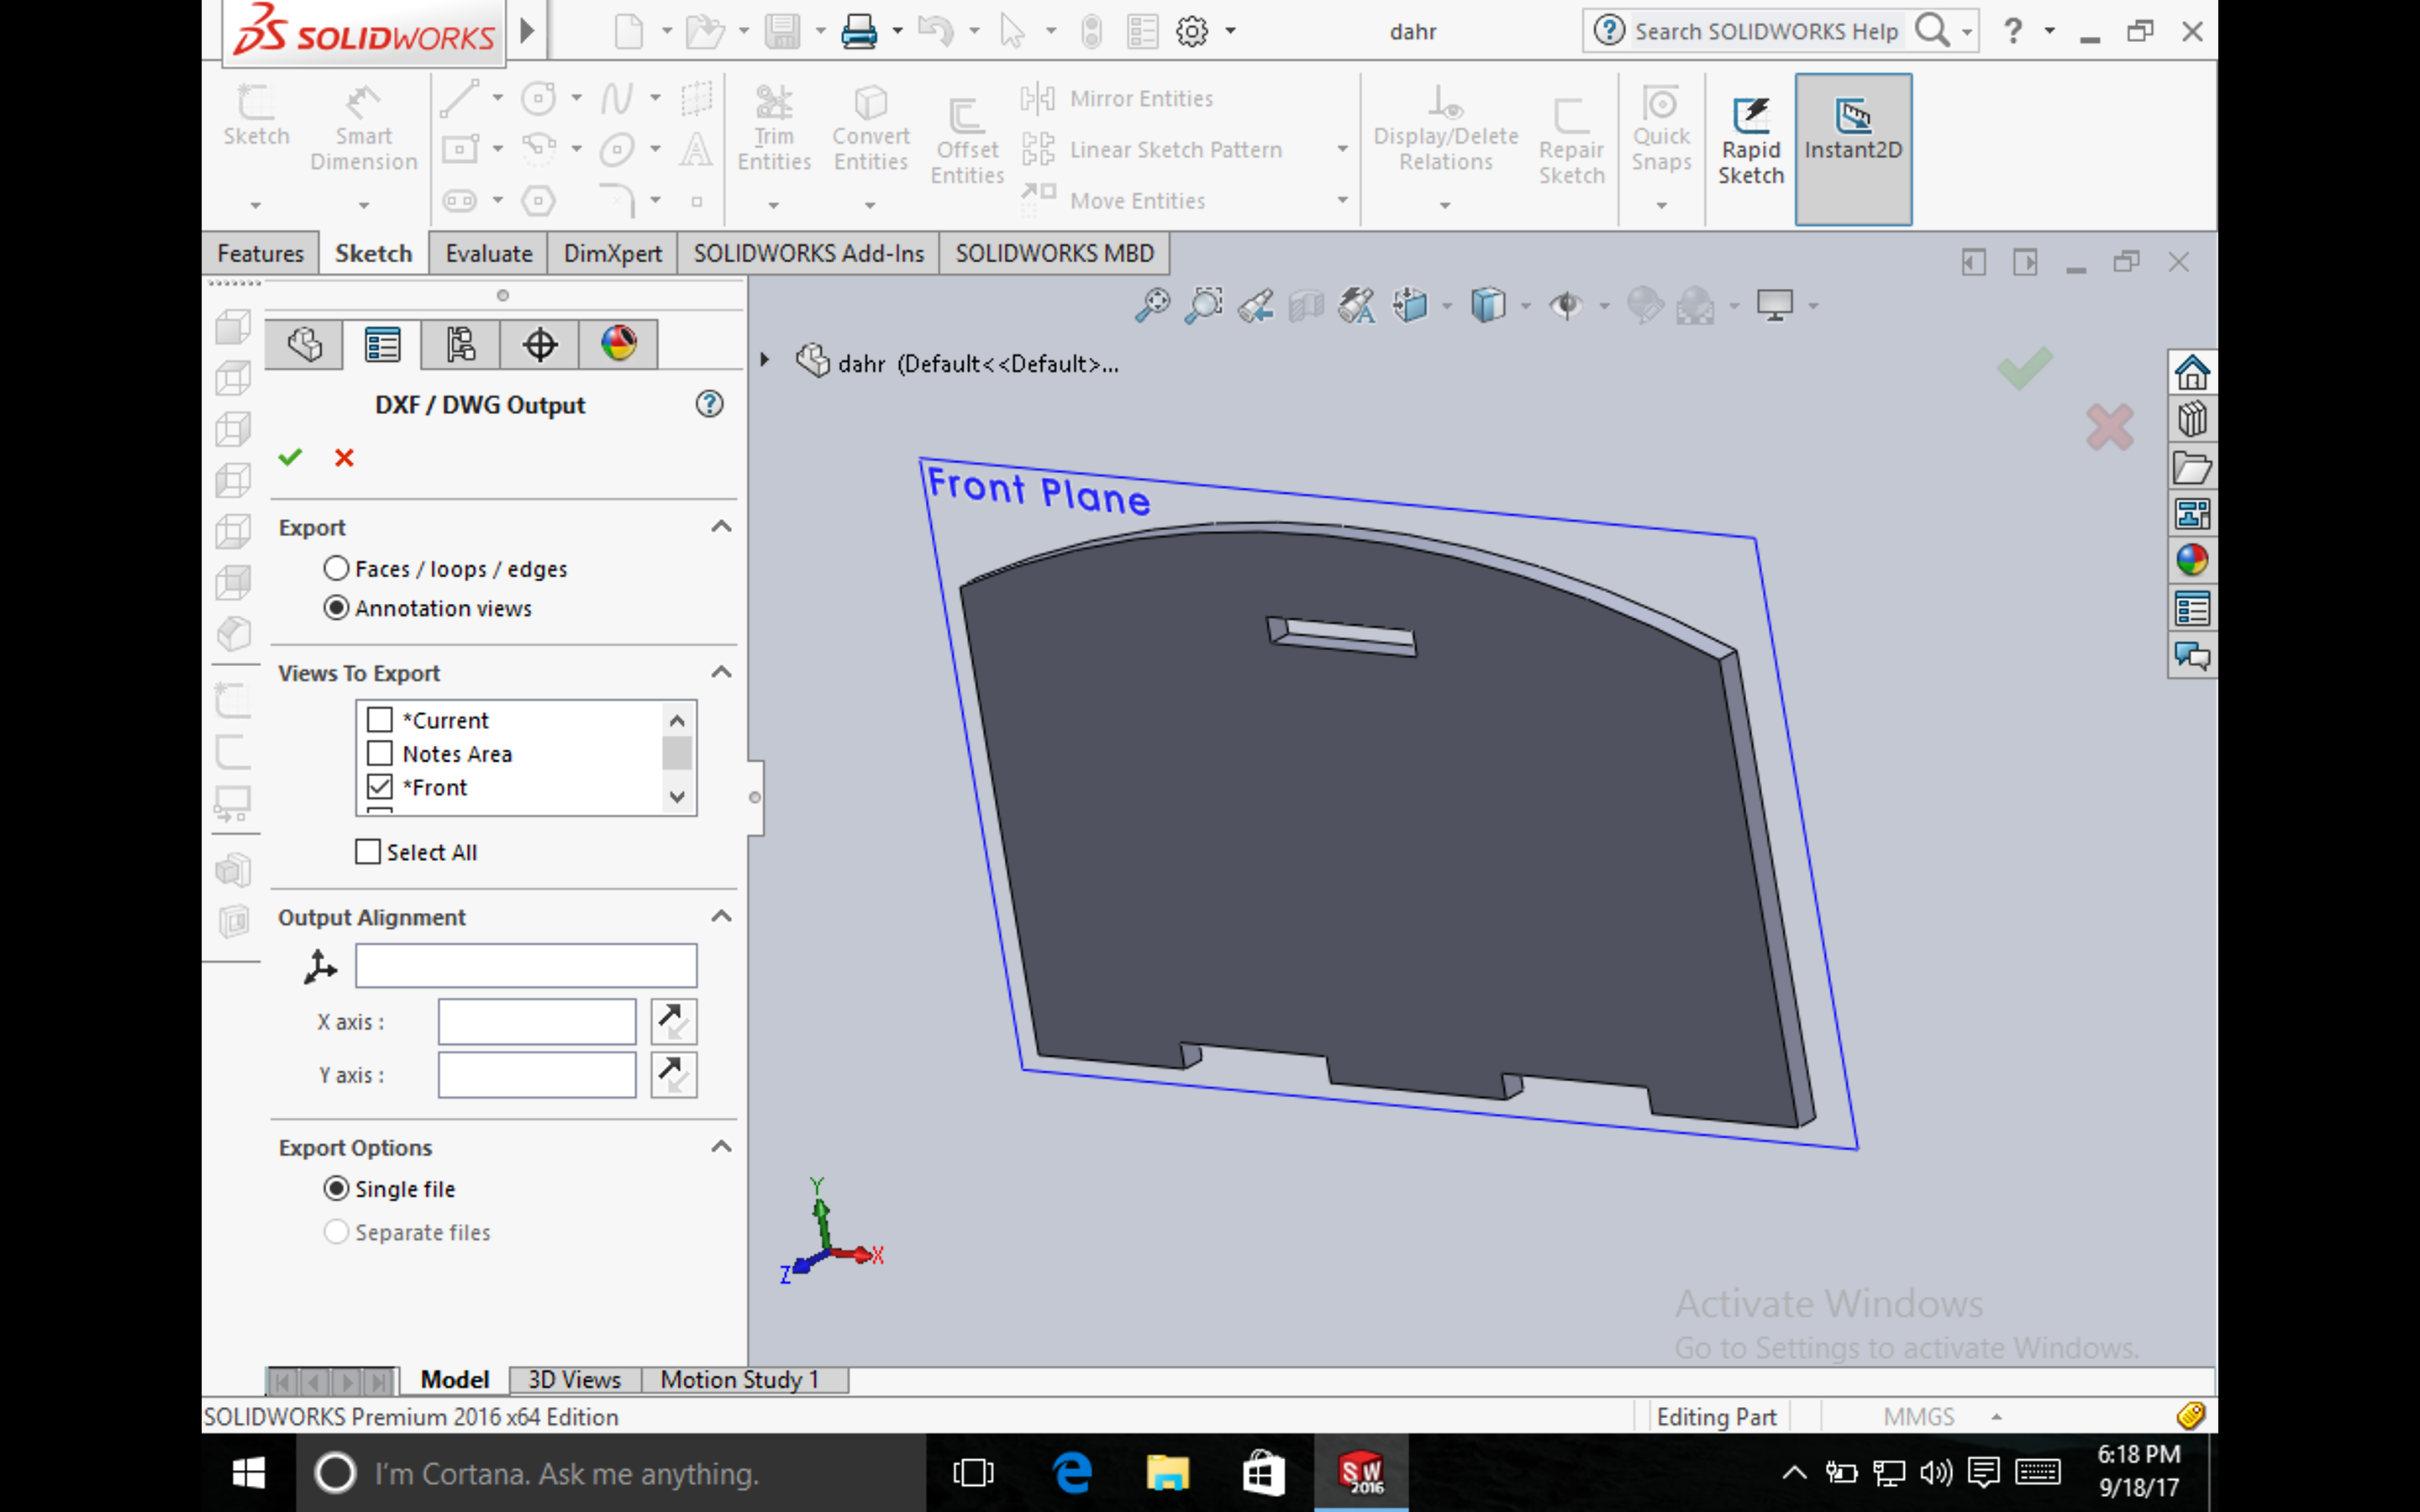
\includegraphics[scale=0.12]{Ch4-Executing/3}
					\caption{}
					\label{D}
					
					\newpage 
					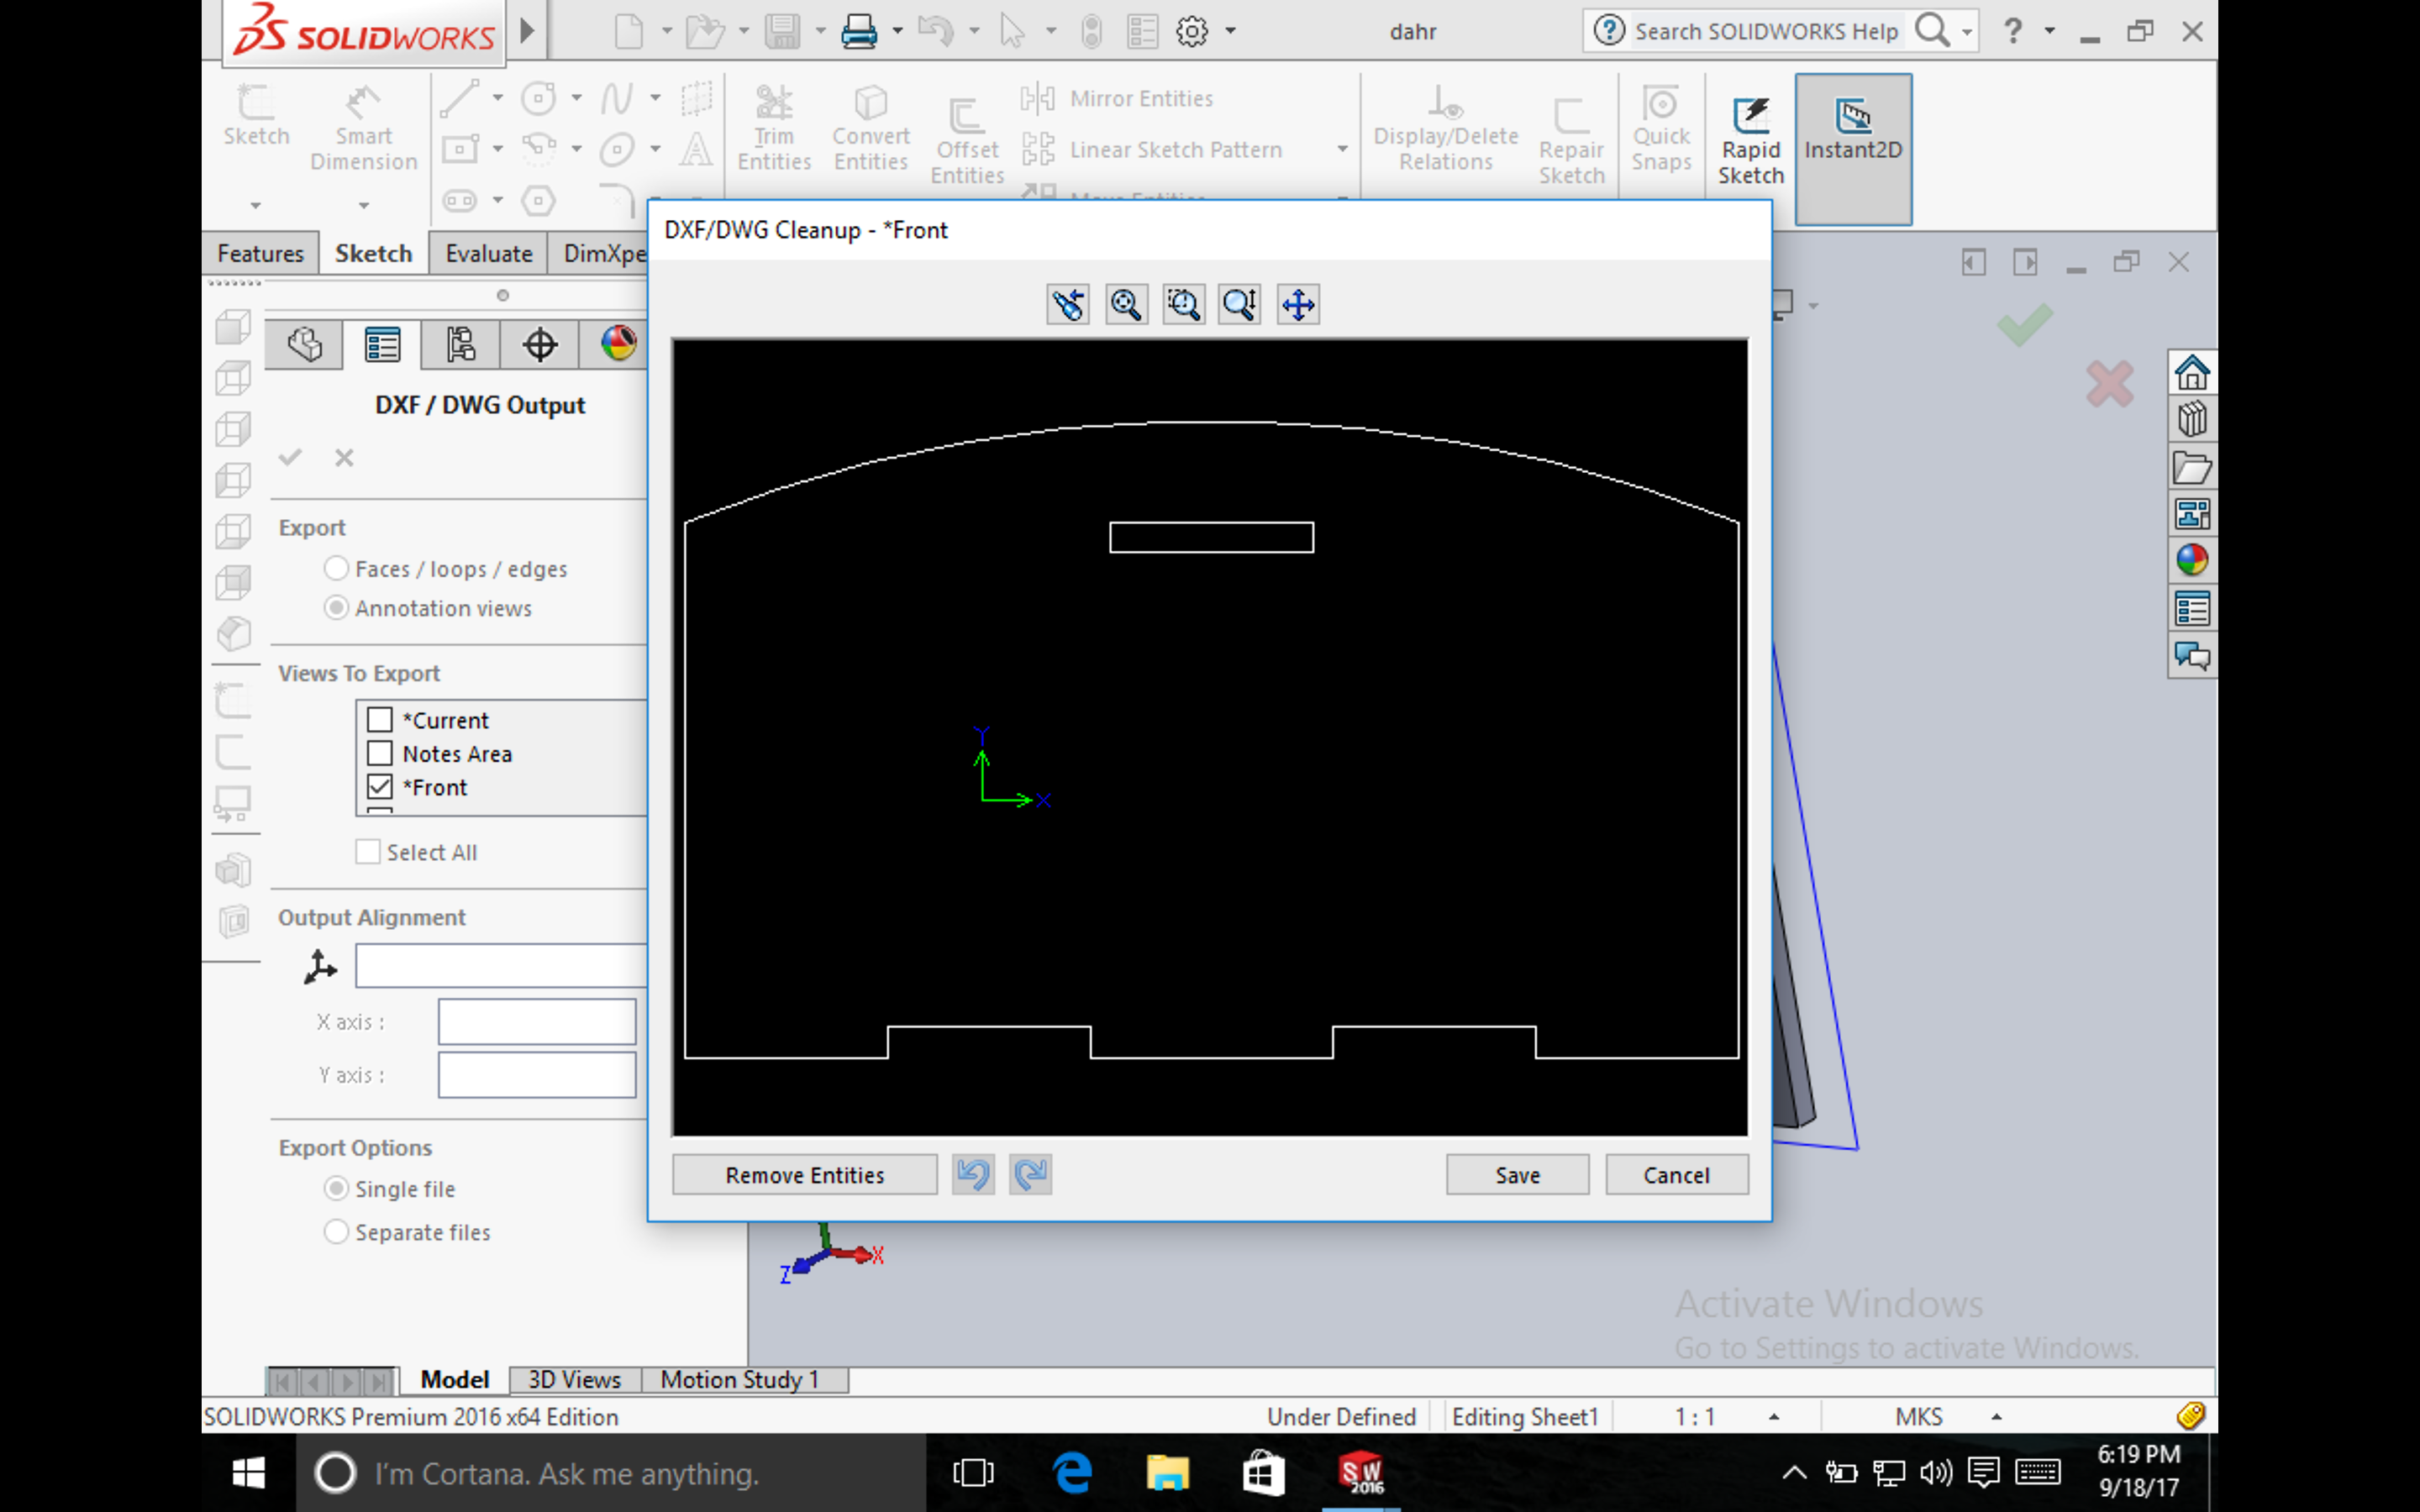
\includegraphics[scale=0.12]{Ch4-Executing/4}
					\caption{}
					\label{E}
					
				\end{subfigure}
				\caption{From Designing To Laser Cutter}
			\end{center}
		\end{figure}
		
		\begin{figure}
			\begin{center}
				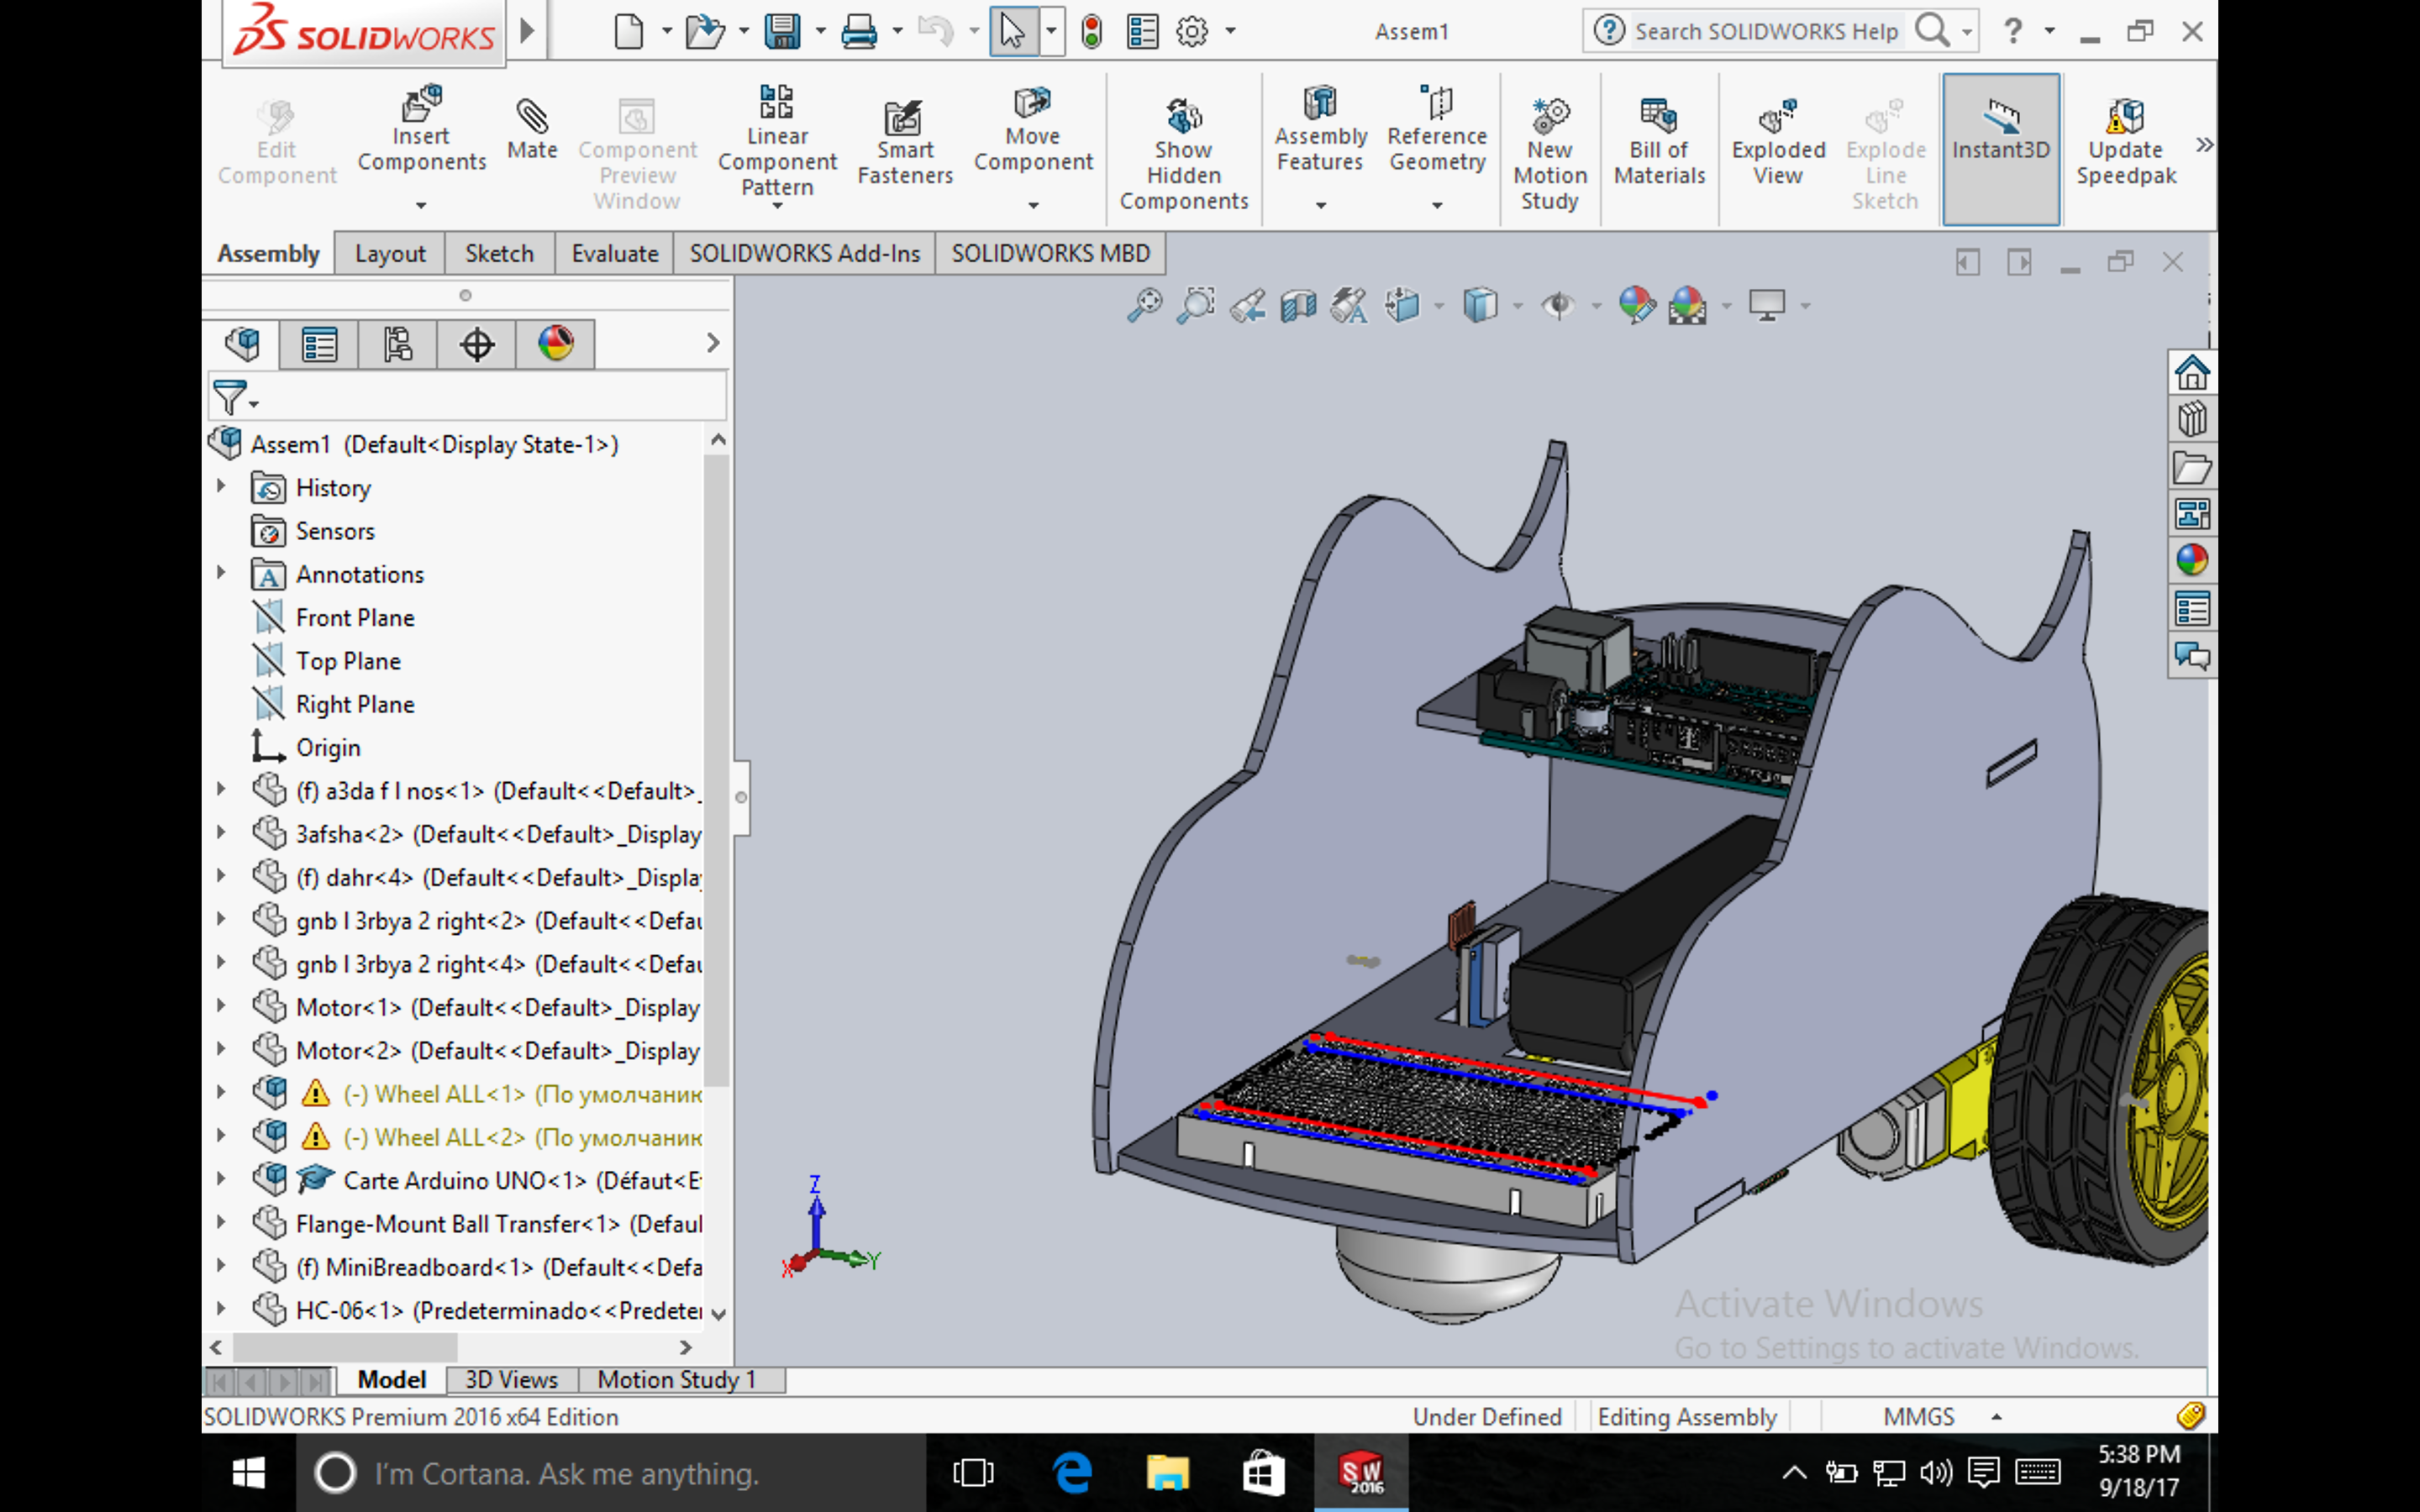
\includegraphics[scale=0.2]{Ch4-Executing/7}
				\caption{Assembly}
			\end{center}
			
		\end{figure}
		
		\begin{figure}[]
			\begin{center}
				\begin{subfigure}[normal]{0.5\textwidth}
					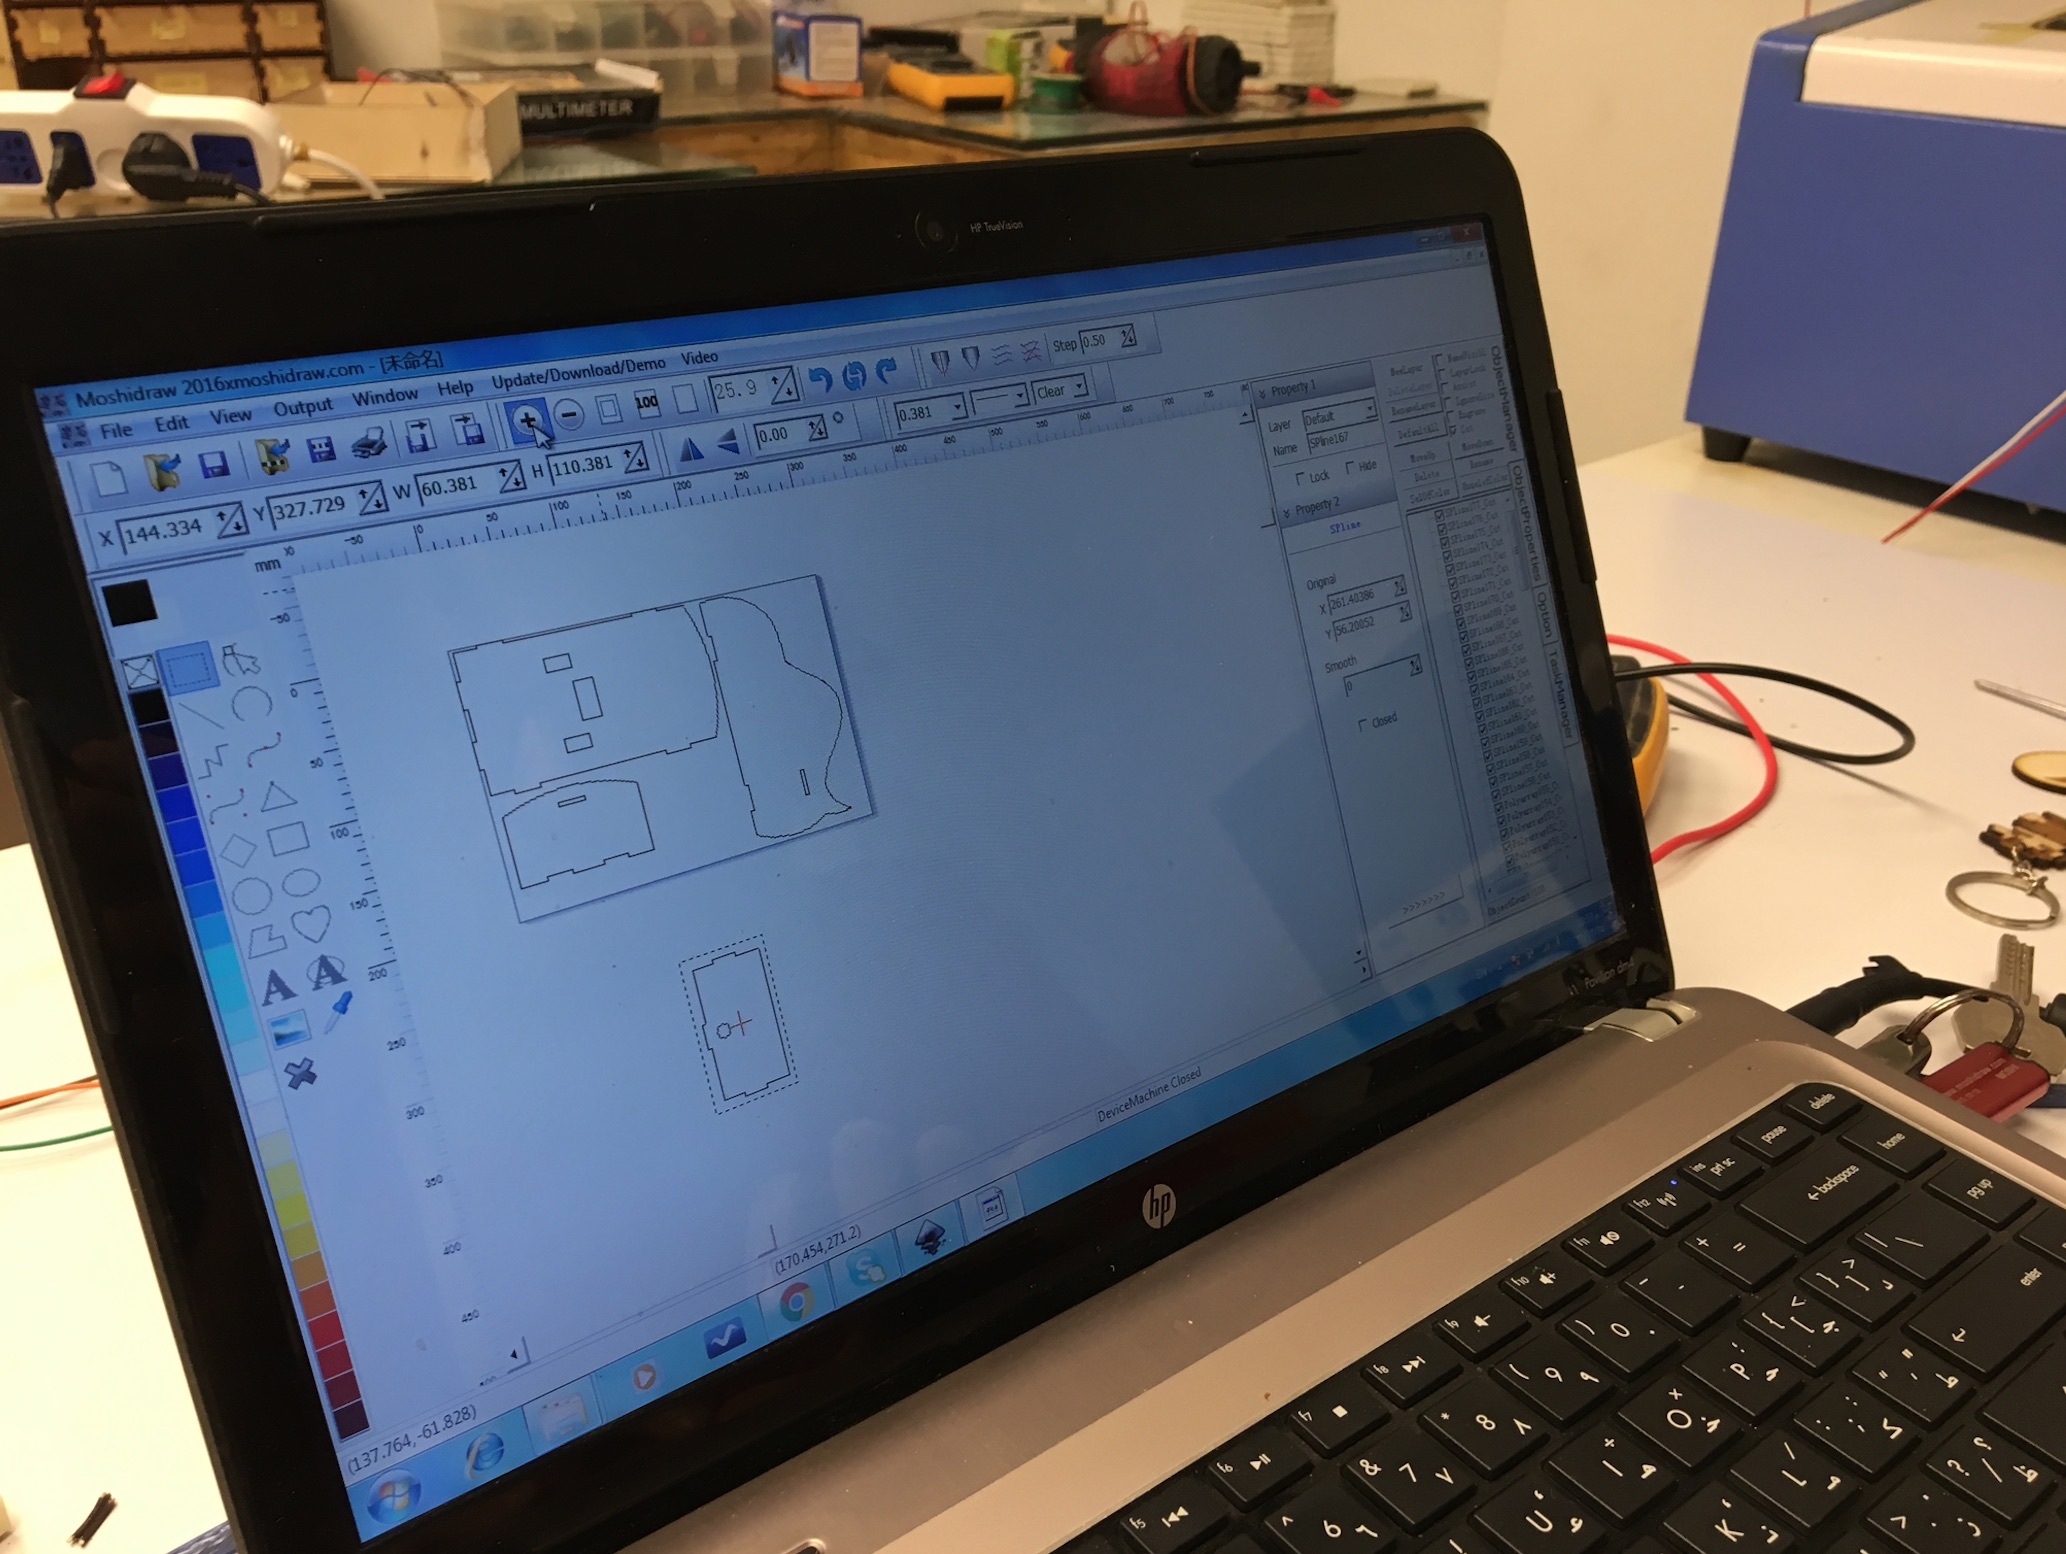
\includegraphics[scale=0.12]{Ch4-Executing/5}
					\caption{}
					\label{A}
					
					\includegraphics[scale=0.23]{Ch4-Executing/6}
					\caption{}
					\label{B}	
				\end{subfigure}
				\caption{Laser Cutter}
			\end{center}
		\end{figure}

		

	
	\newpage
	\chapter{Conclusion}
	
	We finished with important , critical instructions:
	
		-Time managment is critical.
		
		-Use external power supply with the motors (for more than one ) to  avoid mess up the arduino kit.
		
		-Profishinal coumentaion is very important.
		
		-Confirm using the laser cutting machine.
		
		-Confirm using H-bridge IC
		
		 
	
	\newpage
	\begin{appendix}
		\listtablename{ References} \\
			%\cite{Arduino}
	\end{appendix}
	
	
	\begin{appendix}
		\listoffigures
		%\listoftables
	\end{appendix}
	
	\begin{newpage}
		\maketitle
		\textbf{\Huge References	}
		\\ \\ $https://en.wikipedia.org/wiki/Autonomous_robot$ 
		\\$https://www.youtube.com$ 
		\\$https://www.arduino.cc$
		
	\end{newpage}


\end{document}